% !TeX root = probability.tex

%%%%%%%%%%%%%%%%%%%%%%%%%%%%%%%%%%%%%%%%%%%%%%%%%%%%%%%%%%%%%%%%

\documentclass[12pt,a4paper,leqno]{article}

\usepackage{verbatim}
\usepackage{url}
\usepackage{fancyhdr}
\usepackage{graphicx}
\usepackage{bm}

\graphicspath{{../images/}}

% TikZ package
\usepackage{tikz}
\usetikzlibrary{arrows.meta,shapes}
\tikzset {>=Stealth}

% Polyglossia Hebrew (main) and English (other)
\usepackage{polyglossia}  
\setmainlanguage{hebrew}
\setotherlanguage{english}

% Fonts: David for Hebrew, Palatino/Courier for English
\newfontfamily{\hebrewfont}{David}[Script=Hebrew]
\newfontfamily{\englishfont}{Palatino Linotype}
\newfontfamily{\englishfonttt}{Courier New}
\newfontfamily{\hebrewfonttt}{Courier New}

% Abbreviations for backwards compatibility with babel
\renewcommand*{\L}[1]{\textenglish{\small #1}}
\newcommand*{\R}[1]{\texthebrew{#1}}

% Use fancyhdr to make all page numbers uniform
\pagestyle{fancy}
\fancyhead{}
\renewcommand{\headrulewidth}{0pt}
\renewcommand{\footrulewidth}{0pt}
\fancyfoot[C]{$\thepage$}

% Displaystyle for fractions and combinations
\newcommand*{\disfrac}[2]{\displaystyle\frac{#1}{#2}}
\newcommand*{\dischoose}[2]{\displaystyle{#1 \choose #2}}

\newcommand*{\bover}[1]{\bm{\overline{#1}}}
\newcommand*{\erh}[1]{\renewcommand{\arraystretch}{#1}}

% Reduce space around c column in eqnarray*
\newenvironment{eqn}
  {\addtolength{\arraycolsep}{-3pt}\begin{eqnarray*}}
  {\end{eqnarray*}}
  
% Reduce space around c column in eqnarray with labels
\newenvironment{eqnlabels}
  {\addtolength{\arraycolsep}{-3pt}
   \begin{eqnarray}}
  {\end{eqnarray}}

% Use english equation numbers in hebrew document
\renewcommand{\theequation}{\L{\arabic{equation}}}

% Allow pages with larger floats
\renewcommand{\floatpagefraction}{.8}

% Layout
\textwidth=155mm
\textheight=230mm
\topmargin=0pt
\headheight=0pt
\oddsidemargin=0mm
\evensidemargin=0mm
\headsep=0pt
\parindent=0pt
\renewcommand{\baselinestretch}{1.1}
\setlength{\parskip}{0.3\baselineskip plus 1pt minus 1pt}

%\includeonly{}

\begin{document}
% !TeX root = probability.tex

\selectlanguage{hebrew}

\thispagestyle{empty}

\begin{center}
\textbf{\LARGE בחינות בגרות בהסתברות}
\end{center}

\bigskip
\bigskip

\begin{center}
\textbf{\Large מוטי בן-ארי}

\bigskip

\url{http://www.weizmann.ac.il/sci-tea/benari/}
\end{center}

\begin{center}	
\begin{bfseries}
\bigskip
\bigskip

\R{גרסה} \L{1.0} 

\bigskip

\today

\end{bfseries}
\end{center}

\vfill

\selectlanguage{english}

\begin{small}
\begin{center}
\copyright{}\ 2022 \R{מוטי בן-ארי}
\end{center}

This work is licensed under a Creative Commons Attribution-ShareAlike 4.0 International License:
\url{http://creativecommons.org/licenses/by-sa/4.0/}.
\end{small}

\bigskip

\begin{center}

\includegraphics[width=.2\textwidth]{../by-sa.png}
\end{center}

\newpage

\selectlanguage{hebrew}

\thispagestyle{empty}

\tableofcontents

\newpage

\section*{מבוא}
\addcontentsline{toc}{section}{\large מבוא}

חוברת זו כוללת פתרונות לכל השאלות על הסתברות של בחינות הבגרת (שאלון 
$806 / 581$)
מהשנים תשע"ד עד תשפ"ב. 
הדגשים בפתרונות הם:
\begin{itemize}
\item 
זיהוי מוקפד של המאורעות.

\item
הנמקה של בחירת שיטות לחישוב ולהצגת החישוב: עץ, טבלה, ברנולי, בינום, עם דגש מיוחד על הבנת הניסוחים הרבים המכוונים להסתברות מותנית.
\item
לא הססתי לכלול תיאור של מקרים בהם הסתבכתי בפתרון!
\item
בסוף החוברת נמצא סעיף "המלצות" המסכם לקחים מהפתרונות.
\item
החוברת מופצת עם רישיון המאפשר העתקה חופשית. ניתן להוריד את המסמכים ב-%
\L{PDF}
מ:
\begin{center}
\selectlanguage{english}
\url{https://github.com/motib/bagrut}
\selectlanguage{hebrew}
\end{center}
שם נמצא גם קוד המקור ב-%
\L{\LaTeX{}}.
המסמך בעברית ויש להשתמש ב-%
\L{\XeLaTeX{}}
ולא ב-%
\L{pdflatex}.
\end{itemize}

\textbf{סימון המאורעות}
אני מקפיד עם סימון מאורעות כי לדעתי זה מקל על הבנת החישובים לעומת שימוש בשפה טבעית. הסימון גם מעודד חשיבה לזיהוי מוקפד של המאורעות. למשל:
\begin{quote}
נסמן ב-%
$N$ \L{(neta)}
ניצחון של נטע במשחק.
\end{quote}
כאשר מבקשים גם את מספר הנצחונות של נטע נשתמש בסימון כגון
$N=4$
או
$N\geq 5$.\footnote{$N\geq 5$
הוא למעשה משתנה אקראי שערכו גדול או שווה ל-$5$, אבל המונח לא נמצא בתכנית הלימודים.}


% !TeX root = probability.tex

%%%%%%%%%%%%%%%%%%%%%%%%%%%%%%%%%%%%%%%%%%%%%%%%%%%%%%%%%%%%%

\addcontentsline{toc}{section}{\large בחינות ופתרונות}

\section{קיץ תשע"ח מועד ב}

\begin{center}
\selectlanguage{english}
\hspace*{8em}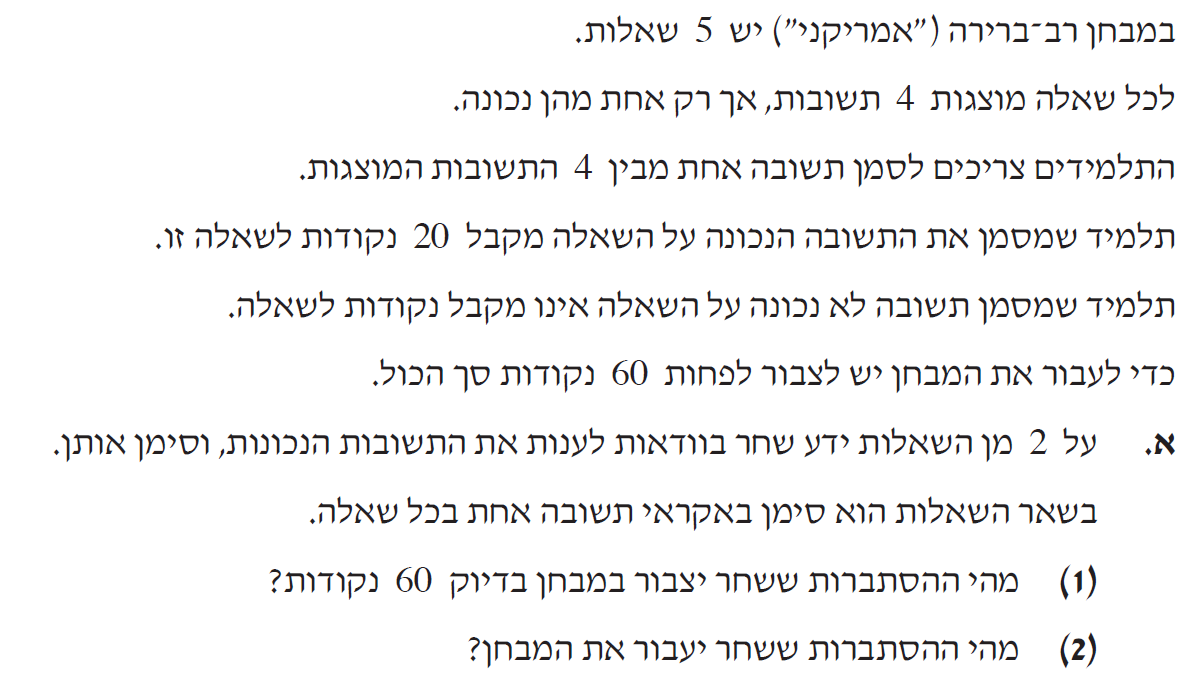
\includegraphics[width=.7\textwidth]{summer-2018b-3a}
\hspace*{-2.2em}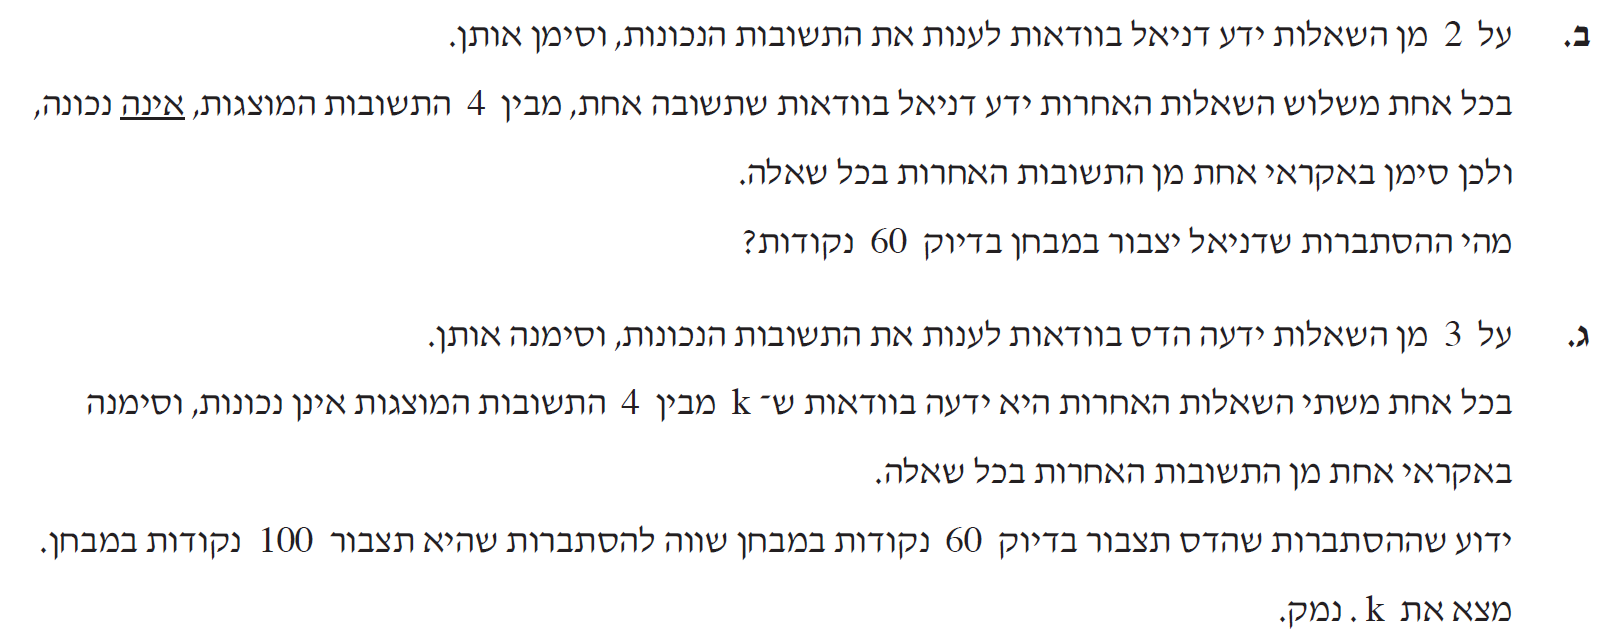
\includegraphics[width=\textwidth]{summer-2018b-3b}
\end{center}

המאורועות הם מספר הנקודות הצברות על ידי התלמידים.

השאלה מתארת הצלחות וכשלונות במתן לתשובות על המבחן ושואלת על מספר ההצלחות והכשלונות. לכן הפתרון ישתמשמ בנוסחת ברנולי.

\textbf{סעיף א}

1. שחר ידע שהוא ענה נכון על שתי שאלות ולכן כדי לקבל ציון
$60$
עליו לענות על בדיוק אחת משלושת השאלות האחרות. ההסתברות לענות נכון על שאלה היא 
$\frac{1}{4}$
ולפי נוסחת ברנולי:
\[
{3 \choose 1}\left(\frac{1}{4}\right)\left(\frac{3}{4}\right)^2=\frac{27}{64}\,.
\]
2. כדי לעבור את המבחן עליו לצבור לפחות שלוש תשובות נכונות. להסתברות מהסעיף הקודם יש להוסיף את ההסתברויות של ארבע וחמש תשובות נכונות:
\[
\frac{27}{64}+{3 \choose 2}\left(\frac{1}{4}\right)^2\left(\frac{3}{4}\right)^1+{3 \choose 3}\left(\frac{1}{4}\right)^3\left(\frac{3}{4}\right)^0=\frac{37}{64}\,.
\]

\newpage

\textbf{סעיף ב}

דניאל צריך לענות נכון על שאלה אחת בדיוק מתוך שלושת השאלות הנותרות. דניאל ידע שתשובה אחת לא נכונה, לכן ההסתברות שהוא ענה נכון על השאלה היא
$\frac{1}{3}$
ולא 
$\frac{1}{4}$
כמו בסעיף הקודם:
\[
{3 \choose 1}\left(\frac{1}{3}\right)\left(\frac{2}{3}\right)^2=\frac{4}{9}\,.
\]
\textbf{סעיף ג}

תהי
$p_k$
ההסתברות שהדס ידעה וודאות ש-%
$k$
מתוך 
$4$
תשובות לא נכונות. ההסתברות שהיא שהיא צריכה לבחור תשובה באופן אקראי היא המשלים
$1-p_k$.
כדי לקבל ציון
$60$
היא צריכה לענות נכון על אפס מתוך שתי השאלות הנוספות וכדי לקבל ציון 
$100$
היא צריכה לענות נכון על כל השאלות הנכונות. נשווה את שתי ההסתברויות המתקבלות מנוסחת ברנולי:
\begin{eqnarray*}
{2 \choose 0}p_k^0(1-p_k)^2 &=& {2 \choose 2}p_k^2(1-p_k)^0\\
(1-p_k)^2 &=& p_k^2\\
p_k&=&\frac{1}{2}\,,
\end{eqnarray*}
כאשר השתמשנו ב-%
${n\choose 0}={n\choose n}=1$
ו-%
$p^0=(1-p)^0=1$.

 ההסתברות שהיא ענתה תשובה נכונה לשאלה אחת היא
$p_k=\displaystyle\frac{1}{4-k}$
ולכן 
$k=2$.

\textbf{פתרון שני}

אם לא היינו מגדירים את הסימון
$p_k$
היינו מקבלים מפישוט השוויון של נוסחאות ברנולי:
\[
\left(\frac{1}{4-k}\right)^2 =\left(1-\frac{1}{4-k}\right)^2=\left(\frac{3-k}{4-k}\right)^2\,.
\]
נכפיל את שני הצדדים של המשוואה ב-%
$(4-k)^2$
ונקבל את המשוואה ריבועית
$k^2-6k+8=0$
שפתרונותיה הם 
$k=2,k=4$.
הפרמטר
$k$
מוגדר כמספר התשובות שהדס יודעת שהן אינן נכונות, ונתון שתשובה אחת נכונה, כך שיש לפסול את הפתרון
$k=4$
ולבחור
$k=2$.

האפשרות השנייה היא לקחת שורש של שני הצדדים ונקבל שתי משוואות:
\begin{eqnarray*}
\frac{1}{4-k}&=&+\frac{3-k}{4-k}\\
\frac{1}{4-k}&=&-\frac{3-k}{4-k}\,.
\end{eqnarray*}
מהמשוואה הראשונה נקבל
$k=2$.
מהמנה של המשוואה השנייה נקבל 
$k=4$
ונפסול אותו כי הוא מאפס את המכנה.

כל הפתרונות מגיעים לתשובה הנכונה אבל בחירה נכונה של סימון וסדר החישובים יכולים להשפוע על פשטות הפתרון.

%%%%%%%%%%%%%%%%%%%%%%%%%%%%%%%%%%%%%%%%%%%%%%%%%%%%%%%%%%%%%%

\newpage

\section{קיץ תשע"ח מועד א}

\begin{center}
\selectlanguage{english}
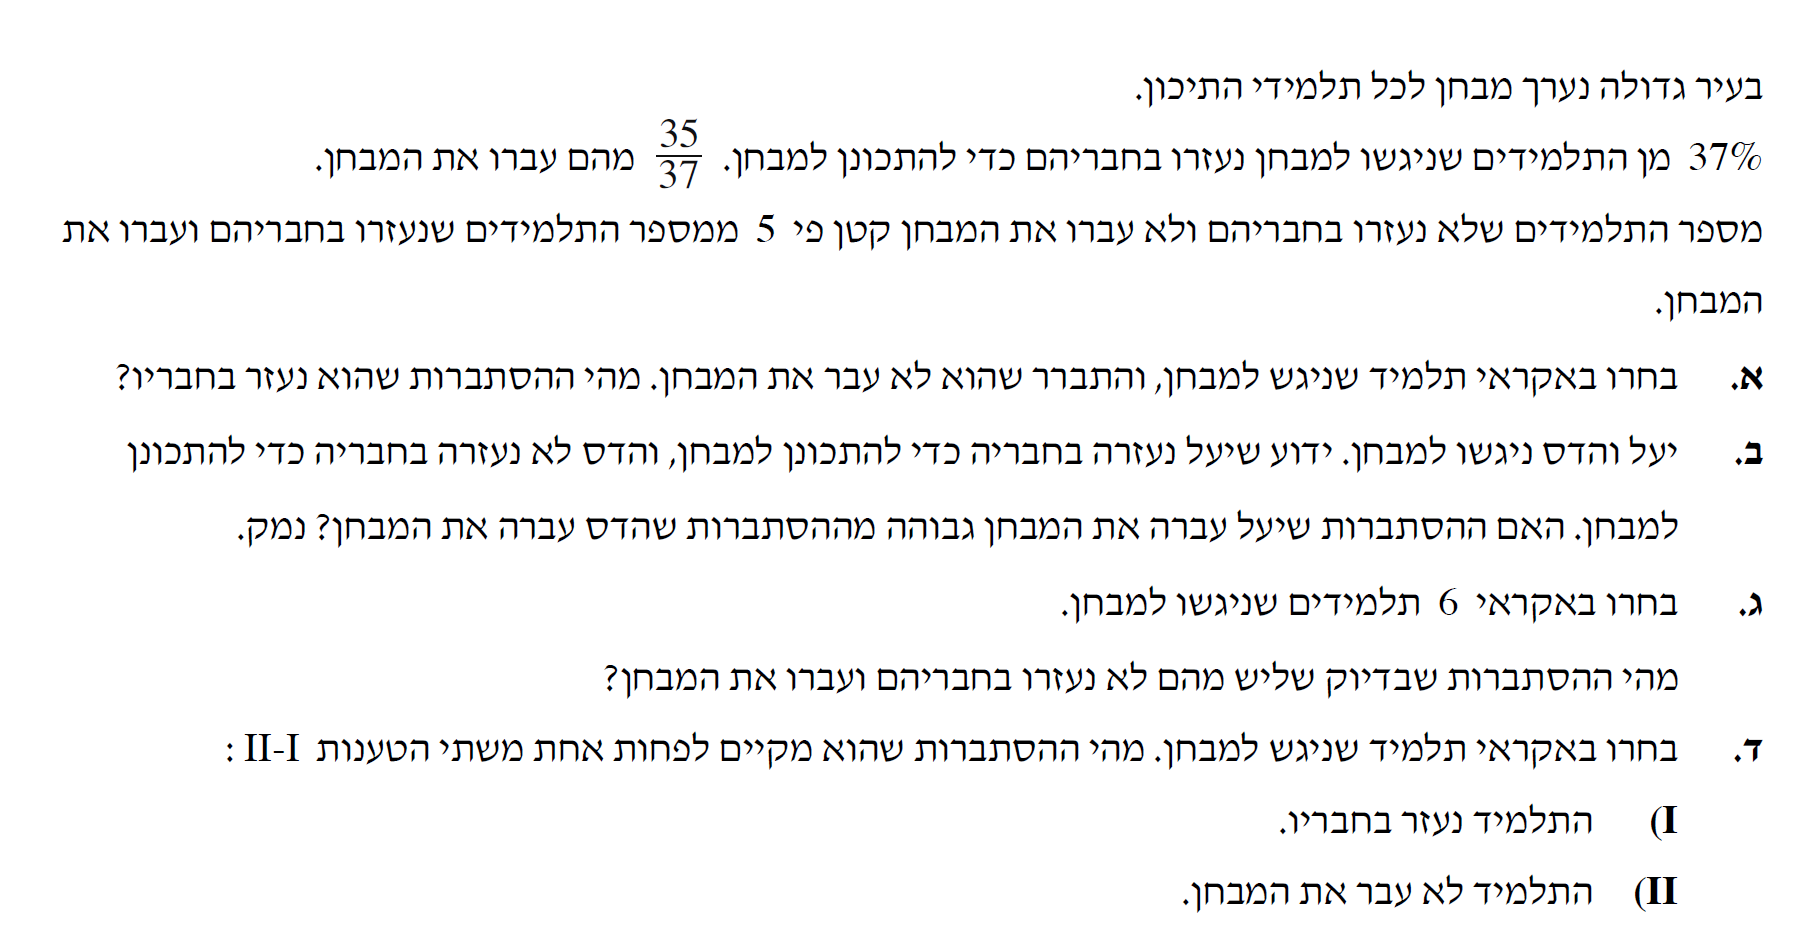
\includegraphics[width=	\textwidth]{summer-2018a-3}
\end{center}

מצאתי שניסוח השאלה מבלבל. כאשר כתוב ש-%
$37\%$
מן התלמידים ניגשו למבחן, הנטייה היא לפרש את זה כ-%
$37$
מתוך
$100$
תלמידים, כאשר אחוז למעשה מבטא יחס:
\[
37\% = \frac{37}{100} = \frac{74}{200} = \frac{18.5}{50} = \cdots\,.
\]
המשפט הבא קובע ש-%
$\frac{35}{37}$
"מהם" עברו את המבחן ואפשר לחשוב שמדובר ב-%
$35$
מתוך
$37$
תלמידים, אולם שוב מדובר ביחס. בשני המקרים יחס הוא הסתברות.

נסמן ב-%
$N$ 
\L{(ne-ezru)}
את התלמידים שנעזרו בחבריהם, וב-%
$A$
\L{(avru)}
את התלמידים שעברו את המבחן. המאורעות מורכבים משתי קבוצות הללו, משלימהם וחיתוכים שלהם, לכן נבחר היעזר בטבלה כדי לייצג את הנתונים. 
לפני שניגש לפתור את השאולות בסעיפים, נמלא את טבלת ההסתברויות לפי המידע הנתון.

\textbf{בניית הטבלה}

נתון ש-%
$P(N)=\frac{37}{100}$.
השימוש במילה
"\textbf{מהם}"
מכוון להסתברות מותנית כך ש:
\[
P(A/N)=\frac{35}{37}
\]
ולכן:
\begin{eqnarray*}
P(A/N) &=& \frac{P(N\cap A)}{P(N)}\\
P(N\cap A) &=& P(A/N)\cdot P(N) = \frac{35}{37}\cdot \frac{37}{100} = \frac{35}{100} = 0.35\,.
\end{eqnarray*}
נשתמש במשלימים להסתברויות ונקבל:
\begin{center}
\selectlanguage{english}
\begin{tikzpicture}[scale=1.25]
\draw (0,0) grid (3,3);
\node at (2.5,3.3) {$\bm{A}$};
\node at (1.5,3.3) {$\bover{A}$};
\node at (3.3,2.5) {$\bm{N}$};
\node at (3.3,1.5) {$\bover{N}$};
\node at (2.5,2.5) {$0.35$};
\node at (0.5,2.5) {$0.37$};
\node at (1.5,2.5) {$0.02$};
\node at (0.5,1.5) {$0.63$};
\node at (0.5,0.5) {$1.0$};
\end{tikzpicture}
\end{center}



בהמשך נתון ש:
\[
P(\overline{N}\cap\overline{A})=\frac{P(N\cap A)}{5}=\frac{0.35}{5}=0.07\,,
\]
וניתן להשלים את הטבלה:
\begin{center}
\selectlanguage{english}
\begin{tikzpicture}[scale=1.25]
\draw (0,0) grid (3,3);
\node at (2.5,3.3) {$\bm{A}$};
\node at (1.5,3.3) {$\bover{A}$};
\node at (3.3,2.5) {$\bm{N}$};
\node at (3.3,1.5) {$\bover{N}$};
\node at (2.5,2.5) {$0.35$};
\node at (0.5,2.5) {$0.37$};
\node at (1.5,2.5) {$0.02$};
\node at (0.5,1.5) {$0.63$};
\node at (0.5,0.5) {$1.0$};
\node at (1.5,0.5) {$0.09$};
\node at (2.5,0.5) {$0.91$};
\node at (1.5,1.5) {$0.07$};
\node at (2.5,1.5) {$0.56$};
\end{tikzpicture}
\end{center}

\smallskip

\textbf{סעיף א}

הניסוח "בחרו 
$\ldots$
תלמיד 
$\ldots$
שלא עבר את המבחן. מה ההסתברות
\textbf{שהוא}
נעזר בחבריו?" מכוון להסתברות מותנית:
\[
P(N/\overline{A})=\frac{P(N\cap \overline{A})}{P(\overline{A})}=\frac{0.02}{0.09}=\frac{2}{9}\,.
\]
\textbf{סעיף ב}

הניסוח
\textbf{"ידוע ש"}
מכוון להסתברות מותנית.

עבור יעל ההסתברות המותנית היא:
\[
P(A/N)=\frac{P(A \cap N)}{P(N)}=\frac{0.35}{0.37}=0.9459\,,
\]
ועבור הדס ההסתברות המותנית היא:
\[
P(A/\overline{N})=\frac{P(A\cap \overline{N})}{P(\overline{N})}=\frac{0.56}{0.63}=0.8889\,.
\]
ליעל הסתברות גבוהה יותר לעבור את המבחן.

\smallskip

\textbf{סעיף ג}

שליש (לא שלושה!) של שש הוא שניים. המילה "בדיוק" מכוון לנוסחת
ברנולי הערך
$P(\overline{N}\cap A)=0.56$
נמצא בטבלה ולפי נוסחה ברנולי ההסתברות היא:
\[
{6 \choose 2}(0.56)^2 (1-0.56)^4=0.1763\,.
\]
\textbf{סעיף ד}

הניסוח
"\textbf{לפחות אחת}"
משתי הטענות
\L{I, II}
אומר שמאורע מורכב משני המאורעות
\L{I, II}
או משניהם. בתרשים להלן שני העגולים המייצגים את שני המאורעות
\L{I, II}
כאשר המאורע "לפחות אחת" מיוצג על ידי כל השטח המקווקו:
\begin{center}
\selectlanguage{english}
\begin{tikzpicture}
\begin{scope}
\clip[draw] (0,0) circle[radius=2];
\foreach \y in {-1.5,-1,-.5,0,.5,1,1.5}
  \draw (-2,\y) -- (2,\y);
\end{scope}
\begin{scope}
\clip[draw] (2.5,0) circle[radius=2];
\foreach \x in {1,1.5,2,2.5,3,3.5,4}
  \draw (\x,-2) -- (\x,2);
\end{scope}
\node at (-2,2.5) {\textrm{I}};
\node at (4.5,2.5) {\textrm{II}};
\node at (1.25,2.5) {\textrm{I}$\:\cap\:$\textrm{II}};
\node at (-3.5,.2) {\textrm{I$-$II}};
\node at (6,.2) {\textrm{II$-$I}};
\draw[->] (1.25,2.2) -- ++(0,-1);
\draw[->] (-3,.2) -- ++(1.7,0);
\draw[->] (5.5,.2) -- ++(-1.7,0);
\draw[->] (-2,2.2) -- +(.6,-.6);
\draw[->] (4.5,2.2) -- +(-.6,-.6);
\end{tikzpicture}
\end{center}
יש שתי דרכים לחשב את ההסתברות. בדרך הראשונה אנו לוקחים את סכום ההסתברויות של שני המאורעים, ומחסירים את ההסתברות של המאורע המשותף כי ספרנו אותו פעמיים, פעם כחלק מהמאורע
\L{I}
ופעם כחלק מהמאורע
\L{II}:
\[
P(\textrm{I} \cup \textrm{II}) = P(\textrm{I}) + P(\textrm{II}) - P(\textrm{I} \cap \textrm{II})\,.
\]
בדרך השניה אנו סופרים כל חלק מהמאורע השותף בנפרד, כאשר הסימון
\L{I-II}
הוא כל האיברים בקבוצה 
\L{I}
שאינם בקבוצה
\L{II}
ולהיפך:
\[
P(\textrm{I} \cup \textrm{II}) = P(\textrm{I}\:-\:\textrm{II}) + P(\textrm{II}\:-\:\textrm{I}) + P(\textrm{I} \cap \textrm{II})\,.
\]
את ההסתברויות לחישוב ניקח מהטבלה. הדרך הראשונה מופיעה מימין והדרך השניה משמאל:
\begin{center}
\selectlanguage{english}
\begin{tikzpicture}[scale=1.25]
\begin{scope}
\draw (0,0) grid (3,3);
\node at (2.5,3.3) {$\bm{A}$};
\node at (1.5,3.3) {$\bover{A}$};
\node at (3.3,2.5) {$\bm{N}$};
\node at (3.3,1.5) {$\bover{N}$};
\node at (2.5,2.5) {$0.35$};
\node at (0.5,2.5) {$0.37$};
\node at (1.5,2.5) {$0.02$};
\node at (0.5,1.5) {$0.63$};
\node at (0.5,0.5) {$1.0$};
\node at (1.5,0.5) {$0.09$};
\node at (2.5,0.5) {$0.91$};
\node at (1.5,1.5) {$0.07$};
\node at (2.5,1.5) {$0.56$};
\draw[ultra thick] (2,2) rectangle +(1,1);
\draw[ultra thick] (1,1) rectangle +(1,1);
\draw[ultra thick] (1,2) rectangle +(1,1);
\end{scope}
\begin{scope}[xshift=6cm]
\draw (0,0) grid (3,3);
\node at (2.5,3.3) {$\bm{A}$};
\node at (1.5,3.3) {$\bover{A}$};
\node at (3.3,2.5) {$\bm{N}$};
\node at (3.3,1.5) {$\bover{N}$};
\node at (2.5,2.5) {$0.35$};
\node at (0.5,2.5) {$0.37$};
\node at (1.5,2.5) {$0.02$};
\node at (0.5,1.5) {$0.63$};
\node at (0.5,0.5) {$1.0$};
\node at (1.5,0.5) {$0.09$};
\node at (2.5,0.5) {$0.91$};
\node at (1.5,1.5) {$0.07$};
\node at (2.5,1.5) {$0.56$};
\draw[ultra thick] (0,2) rectangle +(1,1);
\draw[ultra thick] (1,0) rectangle +(1,1);
\draw[ultra thick] (1,2) rectangle +(1,1);
\end{scope}
\end{tikzpicture}
\end{center}
בשתי הדרכים מקבלים אותה תוצאה:
\begin{eqnarray*}
P(N\cup\overline{A})&=&P(N) + P(\overline{A}) - P(N\cap\overline{A}) = 0.37+0.09-0.02=0.44\\
P(N\cup\overline{A})&=&P(N-\overline{A}) + P(\overline{A}-N) + P(N\cap\overline{A}) = 0.35+0.07+0.02=0.44\,.
\end{eqnarray*}

%%%%%%%%%%%%%%%%%%%%%%%%%%%%%%%%%%%%%%%%%%%%%%%%%%%%%%%%%%%%%

\newpage

\section{חורף תשע"ח}

\begin{center}
\selectlanguage{english}

\includegraphics[width=\textwidth]{winter-2018-3}
\end{center}

\textbf{סעיף א}

נסמן ב-%
$n$
את המספר הפאות של הקוביה של גלית שכתוב עליהן
$1$.
מאורע אחד הוא שמיכל תנצח כי היא מטילה 
$4$
בהסתברות
$\frac{3}{6}$
לא משנה מה גלית מטילה. מאורע שני הוא שמיכל תנצח כי היא מטילה 
$2$
בהסתברות
$\frac{3}{6}$
וגלית מטילה
$1$
בהסתברות
$\frac{n}{6}$.
המאורעות זרים זה לזה ולכן:
\begin{eqnarray*}
P(\textrm{\R{מיכל תנצח}}) &=&
\frac{3}{6}\cdot 1 + \frac{3}{6}\cdot \frac{n}{6}=\frac{7}{12}\\
n &=& 1\,.
\end{eqnarray*}
\textbf{סעיף ב}

גלית תנצח אם היא תנצח ב-%
$3,4,5$
סיבובים. נשמתמש בנוסחת ברנולי כדי לקבל את ההסתברות כתלות של ההסתברות של גלית לנצח בסיבוב אחד שהיא המשלים להסתברות שמיכל תנצח
$1-\frac{7}{12}=\frac{5}{12}$:
\[
P(\textrm{\R{גלית תנצח}})={5\choose 3}\left(\frac{5}{12}\right)^3\left(\frac{7}{12}\right)^2+{5\choose 4}\left(\frac{5}{12}\right)^4\left(\frac{7}{12}\right)^1+{5\choose 5}\left(\frac{5}{12}\right)^5\left(\frac{7}{12}\right)^0=0.3466\,.
\]
\textbf{סעיף ג}

הניסוח
\textbf{אם ידוע}
מכוון להסתברות מותנית. נסמן ב-%
$G$
את המאורע שגלית תנצח במשחק וב-%
$R$
את המאורע שהיא תנצח בסיבוב הראשון:
\[
P(G/R) = \frac{P(G \cap R)}{P(R)}\,.
\]
כדי שגלית תנצח במשחק וגם בסיבוב הראשון, היא חייבת לנצח בסיבוב הראשון וגם ב-%
$2$
או
$3$
או
$4$
מהסיבובים הנותרים:
\begin{eqnarray*}
P(G \cap R)&=&\frac{5}{12}\left[{4 \choose 4}\left(\frac{5}{12}\right)^4 \left(\frac{7}{12}\right)^0+
{4 \choose 3}\left(\frac{5}{12}\right)^3 \left(\frac{7}{12}\right)^1+
{4 \choose 2}\left(\frac{5}{12}\right)^2 \left(\frac{7}{12}\right)^2\right]\\
&=&\textstyle\frac{5}{12}\cdot 0.5534\,.
\end{eqnarray*}
כבר חישבנו ש-%
$P(R)=\frac{5}{12}$
ולכן 
$P(G/R)= 0.5534$.

% !TeX root = probability.tex

%%%%%%%%%%%%%%%%%%%%%%%%%%%%%%%%%%%%%%%%%%%%%%%%%%%%%%%%%%%%%

\selectlanguage{hebrew}

\section{קיץ תשע"ז מועד ב}

\begin{center}
\selectlanguage{english}

\includegraphics[width=.95\textwidth]{summer-2017b-3}
\end{center}
הניסוח "מוציאים באקראי
$\ldots$
\textbf{ולאחר מכן}
שוב מוציאים באקראי" מכוונן לשימוש בעץ. נסמן ב-%
$b$
את מספר הכדורים הכחולים בקופסה
\L{I}.
בתרשים (בעמוד הבא) בכל צומת רשום שני זוגות של מספרים: למעלה רשום מספר הכדורים האדומים ומספר הכדורים הכחולים בקופסה
\L{I}
ומתחתיו מספר הכדורים האדומים ומספר הכדורים הכחולים בקופסה
\L{II}.
על הקשתות רשום צבע הכדור שנשלף ומתחתיו ההסתברות לשלוף את הצבע. למשל, בקשת הראשונה נשלף כדור אדום וההסתברות היא מספר הכדורים האדומים 
$10-b$
חלקי מספר הכדורים בקופסה
$(10-b)+b=10$.

\begin{figure}
\begin{center}
\begin{tikzpicture}
[grow=right,
level 1/.append style={text width=2cm,level distance=5cm,sibling distance=10em},
level 2/.append style={text width=2cm,level distance=7cm,sibling distance=6em}]
\node[text width=2cm] {(10-b,b)\\(3,7)} % root
child {
  node {(10-b,b)\\(3,7)}
    child {
      node {(10-b,b)\\(3,7)}
      edge from parent node[below] {\R{כחול}}
        node[above,xshift=16mm,yshift=-2mm] {$\frac{b}{10}$}
    }
    child {
      node {(9-b,b)\ *\\(4,7)}
      edge from parent node[above] {\R{אדום}}
        node[below,xshift=16mm,yshift=2mm] {$\frac{10-b}{10}$}
    }
    edge from parent node[below] {\R{כחול}} node[above,xshift=8mm,yshift=0mm] {$\frac{b}{10}$}
}
child { 
  node {(9-b,b)\\(4,7)}
    child {
      node {(9-b,b)\ *\\(4,7)}
      edge from parent node[below] {\R{כחול}}
        node[above,xshift=16mm,yshift=-2mm] {$\frac{b}{9}$}
    }
    child {
      node {(8-b,b)\\(5,7)}
      edge from parent node[above] {\R{אדום}}
        node[below,xshift=16mm,yshift=2mm] {$\frac{9-b}{9}$}
    }
    edge from parent node[above] {\R{אדום}} 
      node[below,xshift=8mm,yshift=0mm] {$\frac{10-b}{10}$}
};
\end{tikzpicture}
\end{center}
\end{figure}

\textbf{סעיף א}

הכוכביות בתרשים מסמנות את שני המסלולים המגיעים למאורע המבוקש 
$R1$:
שנשלף כדור אדום אחד בדיוק מקופסה
\L{I}.
שתי השליפות הן זרות זו לזו ולכן ההסתברות היא סכום ההסתברות לאורך כל אחד מהמסלולים, והסתברות זו נתונה בשאלה:
\[
P(R1)=\frac{10-b}{10}\cdot\frac{b}{9} + \frac{b}{10}\cdot\frac{10-b}{10} = \frac{19}{36}\,.
\]
נפשט ונקבל משוואה ריבועית 
$b^2-10b+25=0$
שיש לה פתרון אחד
$b=5$.


\textbf{סעיף ב}

מהמידע הרשום בצד הימיני של התרשים אפשר לראות שמספר הכדורים האדומים שנמצאים בקופסה
\L{II}
הם:
$5,4,4,7$.
נסכם את ההסתברויות של המאורע
$P(R2$,
לשלוף כדור אדום מקופסה
\L{II},
לאורך כל אחד מהמסלולים כאשר קודם נציב 
$b=5$
שמצאנו לעיל:
\[
\begin{array}{rcl}
P(R2)&=&\displaystyle\left(\frac{5}{10}\cdot\frac{4}{9}\right)\left(\frac{5}{12}\right)+
\left(\frac{5}{10}\cdot\frac{5}{9}\right)\left(\frac{4}{11}\right)+\\
&&\displaystyle\left(\frac{5}{10}\cdot\frac{5}{10}\right)\left(\frac{4}{11}\right)+
\left(\frac{5}{10}\cdot\frac{5}{10}\right)\left(\frac{3}{10}\right)
=0.3595\,.
\end{array}
\]

\textbf{סעיף ג}

הניסוח
"\textbf{ידוע ש-}"
מכוון להסתברות מותנית. המאורע החדש הוא
$P(R3)$:
נשארו שלושה כדורים אדומים בקופסה 
\L{II}:
\[
P(R3/R2)=\frac{P(R3\cap R2)}{P(R2)}\,.
\]
את
$P(R2)$
חישבנו בסעיף הקודם.

נשארו שלושה כדורים אדומים רק אם היו אברעה כדורים אדומים לפני הבחירה, מאורע 
$R4$.
ההסתברות 
$P(R4)$
למעשה נתונה
$\frac{19}{36}$,
והיא ההסתברות להגיע לאחד המצבים המסומנים בכוכבית. מכאן שההסתברות של 
$P(R3)$
היא ההסתברות להגיע לאחד מהמצבים כפול ההסתברות לשלוף כדור אדום במצב זה:
\[
P(R3)=P(R4)\cdot \textstyle\frac{4}{11}\,.
\]
ההסתברות המותנית הדרושה היא:
\[
P(R3/R2)=\frac{\frac{19}{36}\cdot\frac{4}{11}}{0.3595}=0.53385\,.
\]

%%%%%%%%%%%%%%%%%%%%%%%%%%%%%%%%%%%%%%%%%%%%%%%%%%%%%%%%%%%%%%%%%%%

\section{קיץ תשע"ז מועד א}

\begin{center}
\selectlanguage{english}
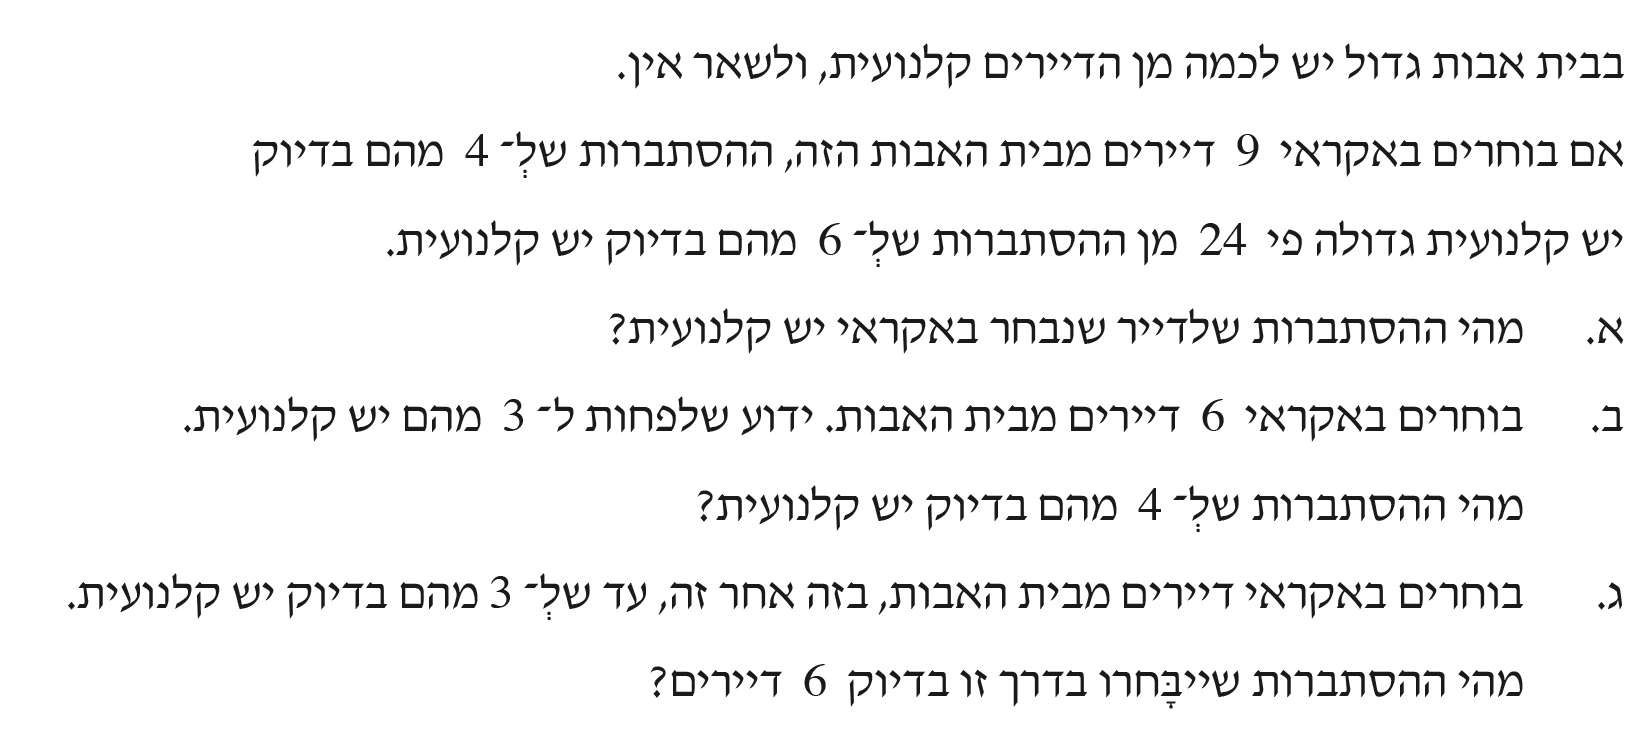
\includegraphics[width=.95\textwidth]{summer-2017a-3}
\end{center}

\textbf{סעיף א}

נסמן ב-%
$D$
את המאורע "לדייר יש קלנועית" ונסמן
$P(D)=p$.
לפי ניסוח השאלה הצלחה היא בחירת דייר עם קלנועית ונמסר מידע על "בדיוק" מספר ההצלחות, ולכן נשמתש בנוסחת ברנולי לכדי לקבל משוואה במשתנה 
$p$:
\begin{eqnarray*}
{9\choose 4} p^4 (1-p)^5&=&24 {9\choose 6} p^6 (1-p)^3\\
\frac{1}{4}(1-p)^2&=&\frac{24}{6}p^2\\
15p^2+2p-1&=&0\\
p&=&\frac{1}{5}=0.2\,,
\end{eqnarray*}
כאשר השורש 
$-\frac{1}{3}$
אינו יכול להיות פתרון כי הסתברות חייבת גדול או שווה לאפס.

\textbf{סעיף ב}

נסמן ב-%
$N$
את המאורע של "מספר הדיירים שיש להם קלנועית". הניסוח
"\textbf{ידוע ש-}"
מכוון להסתברות מותנית:
\[
P(N=4/N\ge3) = \frac{P(N=4\cap N\ge 3)}{P(N\ge 3)}\,.
\]
כאשר קבוצה אחת בחיתוך היא תת-קבוצה של השנייה, אפשר לפשט את החיתוך ולהשתמש רק בקבוצה הקטנה יותר. ברור שאם 
$N$
גדול או שווה ל-%
$3$
\textbf{וגם}
$N$
שווה ל-%
$4$
אז
$N$
שווה ל-%
$4$:
\[
P(N=4/N\ge3) =\frac{P(N=4)}{P(N\ge 3)}\,.
\]
לפי נוסחת ברנולי:
\[
P(N=4)={6\choose 4} 0.2^4 (1-0.2)^2= 0.01536\,.
\]
המונה
$P(N\ge 3)$
אפשר לחשב בשתי דרכים. בצורה ישירה:
\begin{eqnarray*}
P(N\ge 3)&=&{6\choose 3}0.2^3(1-0.2)^3+{6\choose 4}0.2^4(1-0.2)^2+\\
&&{6 \choose 5} 0.2^5(1-0.2)^1+ {6 \choose 6} 0.2^6(1-0.2)^0=0.099\,,
\end{eqnarray*}
או לפי המשלים:
\begin{eqnarray*}
P(N\ge 3)=1-P(N<3)&=&
1-0.2^0(1-0.2)^6-{6\choose 1}0.2^1(1-0.2)^5 -\\
&&{6 \choose 2} 0.2^2(1-0.2)^4=0.099\,.
\end{eqnarray*}
התשובה לשאלה היא:
\[
P(N=4/N\ge3) =\displaystyle\frac{P(N=4)}{P(N\ge 3)}=\displaystyle\frac{0.01536}{0.099}=0.15534\,.
\]
\textbf{סעיף ג}

הניסוח 
"\textbf{עד ש}"
אומר שהבחירה 
\textbf{האחרונה} 
תהיה "הצלחה" ושיהיו שתי "הצלחות" בחמשת הבחירות הקודמות. נסמן הצלחה ב-%
$+$
וכישלון ב-%
$-$
ונסדר את הדרישה בשאלה בשורה:
\[
\overbrace{\pm\;\pm\;\pm\;\pm\;\pm}^{2/5}\quad\quad \overbrace{+}^{1/1}
\]
התשובה מתקבלת מנוסחת ברנולי לבחירות הראשונות כפול ההסתברות
$p$
לבחירה האחרונה:
\[
\left[{5\choose 2}0.2^2 (1-.02)^3\right]\cdot 0.2=0.04096\,.
\]

%%%%%%%%%%%%%%%%%%%%%%%%%%%%%%%%%%%%%%%%%%%%%%%%%%%%%%%%%%%%%

\section{חורף תשע"ז}

\begin{center}
\selectlanguage{english}
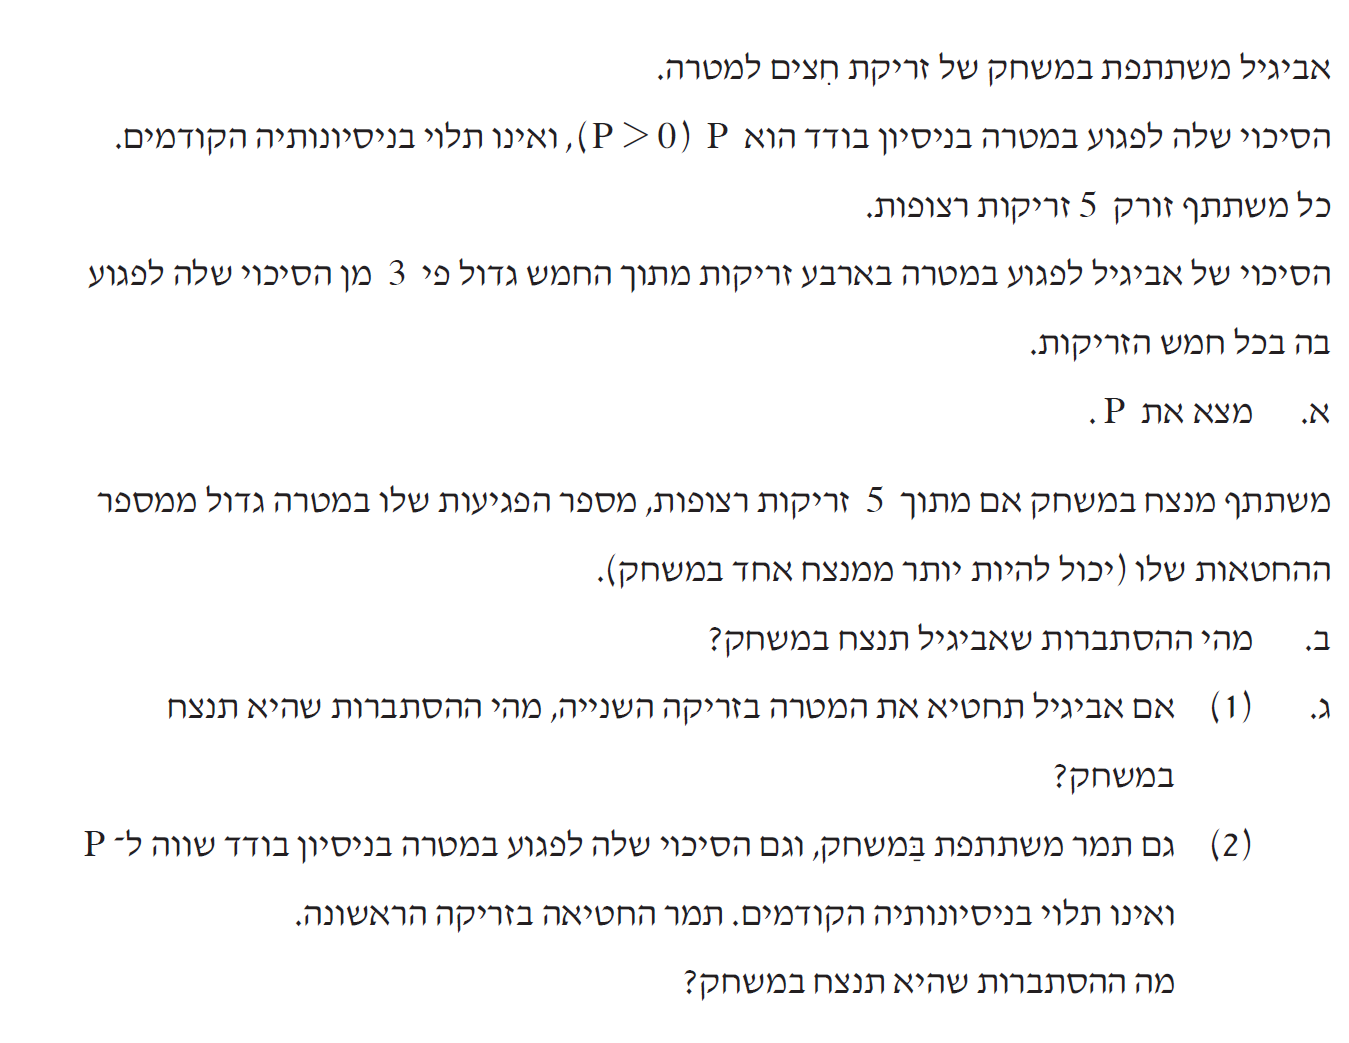
\includegraphics[width=.95\textwidth]{winter-2017-3.png}
\end{center}

\textbf{סעיף א}

נסמן ב-%
$A$
את המאורע "אביגיל פוגעת" ונסמן
$P(A)=p$.
לפי ניסוח השאלה הצלחה היא פגיעה במטרה ונמסר מידע על מספר ההצלחות, ולכן נשמתש בנוסחת ברנולי לכדי לקבל משוואה במשתנה 
$p$:
\begin{eqnarray*}
{5 \choose 4} p^4(1-p)^1 &=& 3{5\choose 5}p^5(1-p)^0\\
5(1-p) &=& 3p\\
p&=&\frac{5}{8}\,.
\end{eqnarray*}

\textbf{סעיף ב}

נסמן ב-%
$N5$
את מספר הפגיעות של אביגיל מתוך חמש זריקות. ניצחון שלה היא 
$N5\geq 3$
וההסתברות היא:
\[
P(N5\geq 3)=
{5 \choose 3}p^3(1-p)^2 + {5 \choose 4}p^4(1-p)^1 + {5 \choose 5}p^5(1-p)^0.
\]
נציב
$p=\displaystyle\frac{5}{8}$
ונקבל
$0.7248$.

\textbf{סעיף ג (1)}

לדעתי ניסוח השאלה לא ברור. אני פירשתי אותה כך: מה ההסתברות של
\textbf{המאורע}
"אביגיל מחטיאה בזריקה השנייה ופוגעת בשלוש או ארבע מהזריקות האחרות"? כותב הבחינה התכוון להסתברות מותנית: "%
\textbf{אם ידוע}
שאביגיל החטיאה בזריקה השנייה, מה ההסתברות שהיא פוגעת בשלוש או ארבע מהזריקות האחרות"?

נסמן ב-%
$T2$
את המאורע שאביגיל מחטיאה בזריקה השנייה, ונסמן ב-%
$N4$
את מספר הפגיעות שלה מתוך ארבע זריקות. ההסתברות המותנית היא:
\[
P(N4\geq 3/T2) = \frac{P(N4\geq 3\cap T2)}{P(T2)}\,.
\]
הזריקות לא תלויות אחת בשנייה ולכן:
\[
P(N4\geq 3/T2) = \frac{P(N4\geq 3)\cdot P(T2)}{P(T2)}=P(N4\geq 3)\,,
\]
ולפי נוסחת ברנולי:
\[
P(N4\geq 3/T2) =P(N4\geq 3)=
{4\choose 4}\left(\frac{5}{8}\right)^4 \left(\frac{3}{6}\right)^0 +{4\choose 3}\left(\frac{5}{8}\right)^3\left(\frac{3}{8}\right)^1 = 0.5188\,.
\]

\textbf{סעיף ג (2)}

ההסתברות של תמר לפגוע זהה להסתברות של אביגיל לפגוע ולכן ניתן להשמתמש בתוצאות שכבר חישבנו. גם לא משנה איזו זריקה החטיאה כי הזריקות בלתי תלויות, ולכן לפי סעיף ג (1) ההסתברות של תמר לנצח היא גם
$0.5188$.

% !TeX root = probability.tex

%%%%%%%%%%%%%%%%%%%%%%%%%%%%%%%%%%%%%%%%%%%%%%%%%%%%%%%%%%%%%

\section{קיץ תשע"ו מועד ב}

\begin{center}
\selectlanguage{english}
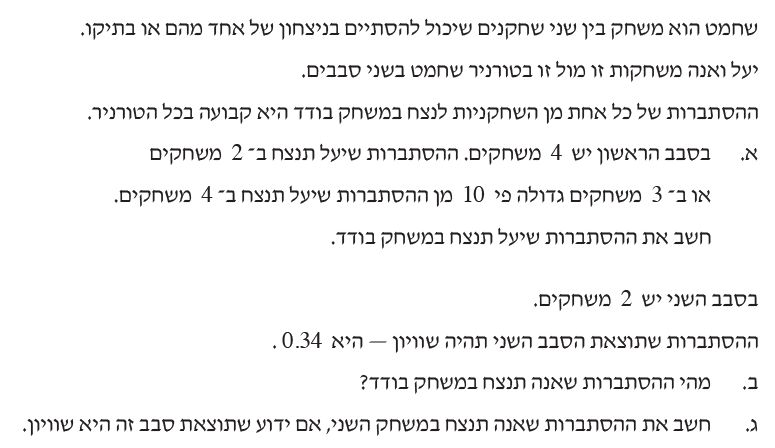
\includegraphics[width=.86\textwidth]{summer-2016b-3}
\end{center}

\textbf{סעיף א}

נסמן את המאורע "יעל תנצח במשחק בודד" ב-%
$Y$ \L{(Yael)}
ונסמן
$y=P(Y)$.
הצלחה מוגדרת על ידי ניצחונות של יעל והשאלה מספקת מידע על מספרי ההצלחות ולכן נשמתמש בנוסחת ברנולי:
\begin{eqnarray*}
{4 \choose 2}y^2(1-y)^2 + {4\choose 3}y^3(1-y) &=& 10\cdot {4\choose 4}y^4(1-y)^0\\
8y^2+8y-6&=&0\\
y&=&\frac{1}{2}\,,
\end{eqnarray*}
ונתעלם מהשורש השני 
$-\frac{3}{2}$
כי הסתברות לא יכולה להיות שלילי.

\textbf{סעיף ב}

נסמן את המאורע "אנה תנצח במשחק בודד" ב-%
$A$ \L{(Anna)}
ונסמן
$a=P(A)$.

נסמן ב-%
$S$ \L{(shivyon)}
את המאורע שתוצאת הסבב השני תהיה תיקו. האפשרויות לקבל שוויון הן ניצחון אחד לאנה וליעל בהסתברות 
$ya+ay$,
או תיקו בשני המשחקים בהסתברות
$(1-(y+a))^2$
כי ההסתברות לתיקו במשחק אחד היא המשלים לסכום ההסתברויות שאחת מהן תנצח. נציב
$y=\frac{1}{2}$
והמידע ש-%
$P(S)=0.34$
ונקבל:
\begin{eqnarray*}
{2 \choose 1}ya + (1-(y+a))^2 &=&P(S)= 0.34\\
a + (\textstyle\frac{1}{2}-a)^2&=&0.34\\
a&=&0.3\,,
\end{eqnarray*}
כאשר נתעלם מהשורש
$-0.3$
כי הסתברות לא יכולה להיות שלילית.

\textbf{סעיף ג}

נסמן את המאורע "אנה תנצח במשחק השני" ב-%
$A2$.

הניסוח
"\textbf{אם ידוע ש-}"
מכוון להסתברות מותנית:
\begin{eqnarray*}
P(A2/S) &=& \frac{P(A2\:\cap\;S)}{P(S)}\\
&=&\frac{ya}{P(S)}=\frac{0.5\cdot 0.3}{0.34}=0.4412\,.
\end{eqnarray*}

ההסתברות לשיוון בסבב השני נתונה. אם אנה תנצח במשחק השני, יהיה שוויון רק אם גם יעל תנצח במשחק הראשון:
\[
\frac{ya}{.34}=\frac{0.5\cdot 0.3}{.34}=0.4412\,.
\]
שימו לב שאם יש שיוון ואנה מנצחת במשחק הראשון, יעל חייבת לנצח במשחק הראשון ולכם המנה היא 
$ya$.

%%%%%%%%%%%%%%%%%%%%%%%%%%%%%%%%%%%%%%%%%%%%%%%%%%%%%%%%%%%%%%

\newpage

\section{קיץ תשע"ו מועד א}

\begin{center}
\selectlanguage{english}
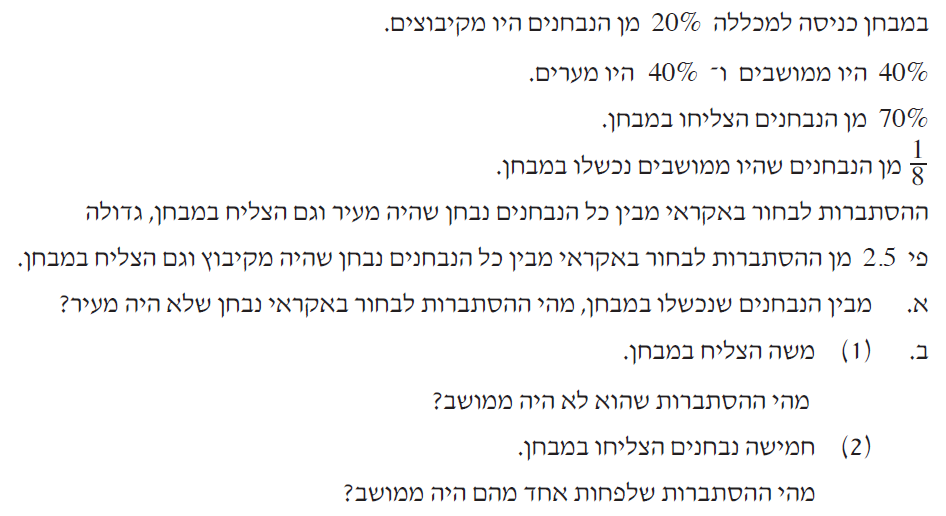
\includegraphics[width=.95\textwidth]{summer-2016a-3}
\end{center}

נסמן את המאורעות השונים בשאלה.
\begin{itemize}
\item $S$ \L{(success)}
הנבחנים שהצליחו.
\item $K$ \L{(kibbutz)} 
נבחנים מקיבוצים.
\item $M$ \L{(moshav)}
נבחנים ממושבים.
\item $E$ \L{(eer)}
נבחנים מערים.
\end{itemize}
ההסתברויות של המאורעות הללו נתונות:
\[
P(K)=0.20,\;P(M)=0.40,\;P(E)=0.40,\;P(S)=0.70\,.
\]
בשאלה שני סוגים של קבוצות: הצלחת הנבחנים ומקום המגורים של הנבחנים ולכן נשתמש בטבלה:
\begin{center}
\selectlanguage{english}
\begin{tikzpicture}[scale=1.25]
\draw (0,0) grid (4,3);
\node at (3.5,3.3) {$K$};
\node at (2.5,3.3) {$M$};
\node at (1.5,3.3) {$E$};
\node at (4.3,2.5) {$S$};
\node at (4.3,1.5) {$\overline{S}$};

\node at (0.5,2.5) {$0.70$};
\node at (0.5,1.5) {$0.30$};
\node at (0.5,0.5) {$1.0$};

%\node at (1.5,2.5) {$0.25$};
%\node at (1.5,1.5) {$0.15$};
\node at (1.5,0.5) {$0.40$};

%\node at (2.5,2.5) {$0.35$};
%\node at (2.5,1.5) {$0.05$};
\node at (2.5,0.5) {$0.40$};

%\node at (3.5,2.5) {$0.10$};
%\node at (3.5,1.5) {$0.10$};
\node at (3.5,0.5) {$0.20$};
\end{tikzpicture}
\end{center}
מידע נוסף שניתן הוא "%
$\frac{1}{8}$
\textbf{מן הנבחנים}
שהיו ממושבים נכשלו במבחן", כאשר הניסוח מכוון להסתברות מותנית. נחשב:
\begin{eqnarray*}
P(\overline{S}/M)&=&P(\overline{S}\cap M) / P(M)\\
P(\overline{S}\cap M)&=&P(\overline{S}/M)\cdot P(M)=\frac{1}{8}\cdot 0.40=0.05\,.
\end{eqnarray*}
הנתון האחרון מתקבל מהפסקאות "ההסתברות לבחור באקראי
\textbf{מבין כל}
הנבחנים נבחן שהיה ב-%
$\cdots$
\textbf{וגם}
הצליח במבחן". הניסוח מכוון לחיתוך הסתברויות, ולכן הנתון הוא
$P(E\cap S)=2.5\cdot P(K\cap S)$.

נחשב את 
$P(S)=0.70$
על ידי סיכום ההסתברויות של המצליחים במבחן בכל מקום מגורים:
\begin{eqnarray*}
P(S)&=&P(K\cap S)+P(M \cap S) + P(K\cap E)\\
0.70&=&P(K\cap S)+ 0.35 + 2.5\cdot P(K\cap S)\\
P(K\cap S)&=&0.10\\
P(E\cap S)&=&0.25\,.
\end{eqnarray*}
נשלים את הטבלה:
\begin{center}
\selectlanguage{english}
\begin{tikzpicture}[scale=1.25]
\draw (0,0) grid (4,3);
\node at (3.5,3.3) {$K$};
\node at (2.5,3.3) {$M$};
\node at (1.5,3.3) {$E$};
\node at (4.3,2.5) {$S$};
\node at (4.3,1.5) {$\overline{S}$};

\node at (0.5,2.5) {$0.70$};
\node at (0.5,1.5) {$0.30$};
\node at (0.5,0.5) {$1.0$};

\node at (1.5,2.5) {$0.25$};
\node at (1.5,1.5) {$0.15$};
\node at (1.5,0.5) {$0.40$};

\node at (2.5,2.5) {$0.35$};
\node at (2.5,1.5) {$0.05$};
\node at (2.5,0.5) {$0.40$};

\node at (3.5,2.5) {$0.10$};
\node at (3.5,1.5) {$0.10$};
\node at (3.5,0.5) {$0.20$};
\end{tikzpicture}
\end{center}
\textbf{סעיף א}

לפי הנוסחה להסתברות מותנית:
\[
P(\overline{E}/\overline{S})=P((K\cup M)/\overline{S}) = \frac{P(K\cap \overline{S})+P(M\cap \overline{S})}{P(\overline{S})}=\frac{0.10+0.05}{0.30}=\frac{1}{2}\,.
\]
\textbf{(1) סעיף ב}

לפי הנוסחה להסתברות מותנית:
\[
P(\overline{M}/S)=P((K\cup E)/S) = \frac{P(K\cap S)+P(E\cap S)}{P(S)}=\frac{0.10+0.25}{0.70}=\frac{1}{2}\,.
\]
\textbf{(2) סעיף ב}

"לפחות אחד ממושב" הוא המשלים ל-"כולם לא מהמושב" ולפי נוסחת ברנולי:
\[
1-P(\overline{M}/S)^5=1-\left(\frac{1}{2}\right)^2=\frac{31}{32}\,.
\]

%%%%%%%%%%%%%%%%%%%%%%%%%%%%%%%%%%%%%%%%%%%%%%%%%%%%%%%%%%%%

\section{חורף תשע"ו}

\begin{center}
\selectlanguage{english}
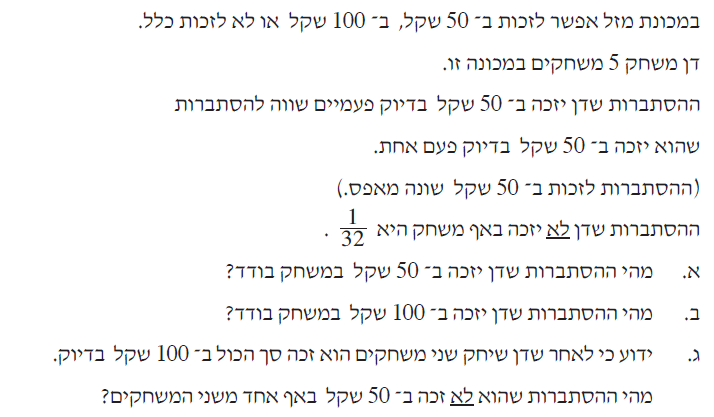
\includegraphics[width=.85\textwidth]{winter-2016-3}
\end{center}

המאורעות הם סכומי הכסף שדן זכה 
$0,50,100$.
נסמן ב-%
$P(n)$
את ההסתברות שדן זכה ב-%
$n$.

\textbf{סעיף א}

הניסוחים "אף אחד" ו-"בדיוק" מכוונים לנוסחת ברנולי. ההסתברות שדן לא זכה (בסכום חיובי) באף אחד מחמישת המשחקים היא 
$P(0)^5=\frac{1}{32}$
ולכן 
$P(0)=\frac{1}{2}$.
לפי המידע הנתון:
\begin{eqnarray*}
{5\choose 2} P(50)^2 (1-P(50))^3 &=& {5\choose 1} P(50) (1-P(50))^4\\
10P(50)&=&5(1-P(50))\\
P(50)&=&\frac{1}{3}\,.
\end{eqnarray*}

\textbf{סעיף ב}

לפי ההסתברות המשלימה:
$P(100) = 1 - P(0) - P(50) = 1-\frac{1}{2}-\frac{1}{3}=\frac{1}{6}$.



\textbf{סעיף ג}

נסמן ב-%
$M2$
את המאורע שדן זכה ב-%
$100$
בשני משחקים ונסמן ב-%
$\overline{50}$
את המאורע שדן לא זכה ב-%
$50$.
הניסוח
"\textbf{ידוע כי}"
מכוון להסתברות מותנית:
\[
P(\overline{50}/M2)=\frac{P(\overline{50}\cap M2)}{P(M2)}
\]
המשחקים מתרחשים אחד אחרי השני ולא לתלויים אחד בשני ולכן ניתן להציג את ההסתברויות בעץ (בעמוד הבא). בסוף כל מסלול רשום המאורעות 
$M2,\overline{50}$
שמתקיימים. ההסתברות המותנית היא:
\[
\frac{\frac{1}{2}\cdot\frac{1}{6} + \frac{1}{6}\cdot \frac{1}{2}}{\frac{1}{2}\cdot\frac{1}{6} + \frac{1}{3}\cdot \frac{1}{3}+ \frac{1}{6}\cdot \frac{1}{2}}  =  \frac{\frac{1}{6}}{\frac{5}{18}}=\frac{3}{5}\,.
\]

\begin{center}
\begin{tikzpicture}
[grow=right,
level 1/.append style={level distance=2cm,
                       sibling distance=7em},
level 2/.append style={level distance=4cm,
                       sibling distance=2.5em}]
\node[left] {$\scriptstyle 0$} % root
child {
  node[right] {$\scriptstyle 100$}
    child {
      node[right] {$\scriptstyle 200\quad \{\overline{50}\}$}
      edge from parent node[below] {$\scriptstyle 1/6$}
    }
    child {
      node[right] {$\scriptstyle 150$}
      edge from parent node[below,near end] {$\scriptstyle 1/3$}
    }
    child {
      node[right] {$\scriptstyle 100\quad \{M2,\overline{50}\}$}
      edge from parent node[above] {$\scriptstyle 1/2$}
    }
    edge from parent node[below,yshift=-2mm] {$\scriptstyle 1/6$}
}
child {
  node[right] {$\scriptstyle 50$}
    child {
      node[right] {$\scriptstyle 150$}
      edge from parent node[below] {$\scriptstyle 1/6$}
    }
    child {
      node[right] {$\scriptstyle 100\quad \{\overline{M2}\}$}
      edge from parent node[below,near end] {$\scriptstyle 1/3$}
    }
    child {
      node[right] {$\scriptstyle 50$}
      edge from parent node[above] {$\scriptstyle 1/2$}
    }
    edge from parent node[below] {$\scriptstyle 1/3$}
}
child {
  node[right] {$\scriptstyle 0$}
    child {
      node[right] {$\scriptstyle 100\quad \{M2,\overline{50}\}$}
      edge from parent node[below] {$\scriptstyle 1/6$}
    }
    child {
      node[right] {$\scriptstyle 50$}
      edge from parent node[below,near end] {$\scriptstyle 1/3$}
    }
    child {
      node[right] {$\scriptstyle 0\quad \{\overline{50}\}$}
      edge from parent node[above] {$\scriptstyle 1/2$}
    }
    edge from parent node[above,yshift=2mm] {$\scriptstyle 1/2$}
}
;
\end{tikzpicture}
\end{center}


% !TeX root = probability.tex

%%%%%%%%%%%%%%%%%%%%%%%%%%%%%%%%%%%%%%%%%%%%%%%%%%%%%%%%%%%%%

%%%%%%%%%%%%%%%%%%%%%%%%%%%%%%%%%%%%%%%%%%%%%%%%%%%%%%%%%%%%%%

\section{קיץ תשע"ה מועד ב}

\begin{center}
\selectlanguage{english}

\includegraphics[width=.85\textwidth]{summer-2015b-3}
\end{center}

\textbf{סעיף א (1)}

נסמן את המאורע "מביא אוכל מהבית" ב-%
$M$ \L{mavi}
ונסמן
$b=P(M)$.
המילה "בדיוק" מכוון לנוסחת ברנולי:
\begin{eqn}
{4 \choose 2} b^2(1-b)^2 &=& 6\cdot {4 \choose 1} b (1-b)^3\\
6b&=&24(1-b)\\
b&=&\frac{4}{5}\,.
\end{eqn}
השאלה שואלת על "אחוז" ולכן התשובה היא
$80\%$.

\textbf{סעיף א (2)}

ההסתברות של "לפחות אחד אבל לא כולם" היא המשלים ל-"לא אפס ולא כולם":
\[
1-\left(\frac{1}{5}\right)^8-\left(\frac{4}{5}\right)^8=0.8322\,.
\]

\textbf{סעיף ב (1)}

נסמן את המאורע "אוכל בקפטריה" ב-%
$C$ \L{(cafeteria)}.
בעץ ההסתברויות בעמוד הבא הכוכבית מראה את מהמסלול עבור המאורע 
$C$
ולכן:
\[
P(C)=\frac{1}{5}\cdot \frac{4}{10} = \frac{2}{25}\,.
\]

\begin{figure}
\begin{center}
\begin{tikzpicture}
[grow=right,
level 1/.append style={level distance=3cm,sibling distance=6em},
level 2/.append style={text width=1cm,level distance=4cm,sibling distance=8em}]
\node[text width=1cm] {} % root
child {
  node {}
    edge from parent node[below,xshift=-5mm,yshift=-3mm] {\R{מביא מהבית}}
      node[above,xshift=3mm,yshift=-4pt] {$\frac{4}{5}$}
}
child { 
  node {}
    child {
      node {$*$}
      edge from parent node[below,xshift=5mm,yshift=-3mm] {\R{אוכל בקפטריה}}
        node[above,xshift=11mm,yshift=-2mm] {$\frac{4}{10}$}
    }
    child {
      node {}
      edge from parent node[above,xshift=5mm,yshift=3mm] {\R{לא אוכל}}
        node[below,xshift=10mm,yshift=2mm] {$\frac{6}{10}$}
    }
    edge from parent node[above,xshift=-4mm,yshift=5mm] {\R{לא מביא מהבית}}
      node[below,xshift=4mm,yshift=2mm] {$\frac{1}{5}$}
};
\end{tikzpicture}
\end{center}
\end{figure}
פתרון זה לא כל כך מוצא חן בעיני כי לא ברור מאיפה צץ העץ שבדרך כלל משמש למאורעות סדרתיות כגון הטלת קוביות מספר פעמים. אני מעדיף פתרון מבוסס הסתברות מותנית ואני חושב שניסוח השאלה היתה צריכה להיות "%
\textbf{מבין}
אלה שלא מביאים אוכל
$60\%$
אינם אוכלים בקפטריה". לפי נוסחת ההסתברות השלמה:
\[
P(C) = P(C/M)P(M) + P(C/\overline{M})P(\overline{M})=
0\cdot 0.8 + (1-0.6)\cdot (1-0.8)=0.4\cdot 0.2=0.08\,.
\]


\textbf{סעיף ב (2)}

נסמן ב-%
$O$ \L{(okhel)}
את המאורע "מביא אוכל. המילה
"\textbf{מבין}"
מכוונת להסתברות מותנית, ונחשב אותה תוך שימוש בעובדה ש-%
$M\subseteq O$
ןלכן
$M\cap O = M$:
\begin{eqn}
P(M/O) &=& \frac{P(M \:\cap\: O)}{P(O)}\\
&=& \frac{P(M)}{P(O)}\\
&=&\frac{\frac{4}{5}}{\frac{4}{5}+\frac{2}{25}}=\frac{10}{11}\,.
\end{eqn}

%%%%%%%%%%%%%%%%%%%%%%%%%%%%%%%%%%%%%%%%%%%%%%%%%%%%%%%%%%%%%

\section{קיץ תשע"ה מועד א}

\begin{center}
\selectlanguage{english}
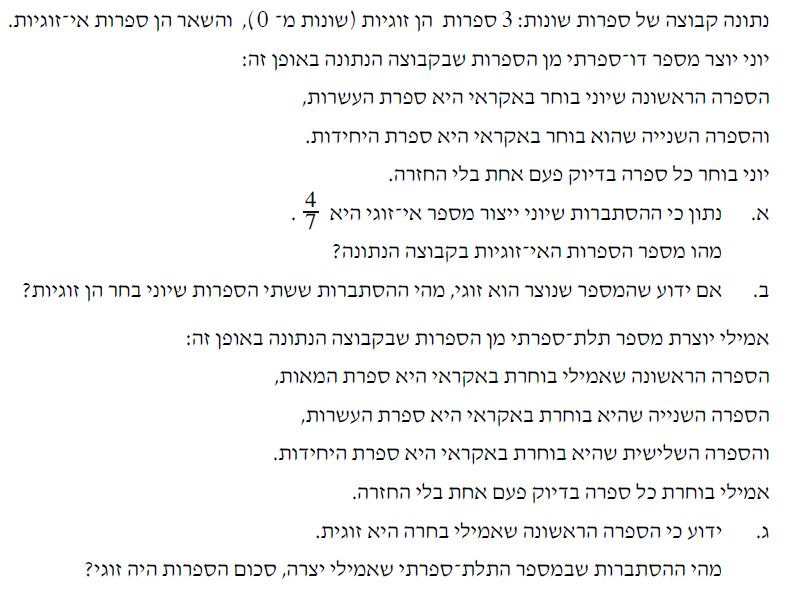
\includegraphics[width=.9\textwidth]{summer-2015a-3}
\end{center}

\textbf{סעיף א}

נסמן את קבוצת הספרות ב-%
$S$ \L{(sifarot)},
קבוצת הספרות הזוגיות ב-%
$Z$ \L{(zugi)},
קבוצת הספרות האי-זוגיות ב-%
$I$ \L{(i-zugi)}.
בחירה של ספרת העשרות ואחר כך ספרת היחידות מכוונת לעץ הסתברויות. במקום לרשום את מספרי הספרות בצמתים וההסתברויות על הקשתות, נפשט את התרשים ונרשום בכל צומת את ההסתברויות שליפת ספרה זוגית או אי-זוגית
$(P(Z=k_1),P(I=k_2))$.

\begin{center}
\begin{tikzpicture}
[grow=right,
level 1/.append style={text width=2cm,level distance=3.5cm,sibling distance=6em},
level 2/.append style={text width=2.5cm,level distance=4.5cm,sibling distance=3.5em}]
\node[text width=2cm] {$\left(\frac{3}{n},\frac{n-3}{n}\right)$} % root
child {
  node {$\left(\frac{3}{n-1},\frac{n-4}{n-1}\right)$}
    child {
      node {$\left(\frac{3}{n-2},\frac{n-5}{n-2}\right)\quad *$}
      edge from parent node[below,xshift=5mm,yshift=-1mm] {\R{אי-זוגי}}
    }
    child {
      node {$\left(\frac{2}{n-2},\frac{n-4}{n-2}\right)$}
      edge from parent node[above,xshift=5mm,yshift=1mm] {\R{זוגי}}
    }
    edge from parent node[below,yshift=-1mm] {\R{אי-זוגי}}
}
child { 
  node {$\left(\frac{2}{n-1},\frac{n-3}{n-1}\right)$}
    child {
      node {$\left(\frac{2}{n-2},\frac{n-4}{n-2}\right)\quad *$}
      edge from parent node[below,xshift=5mm,yshift=-1mm] {\R{אי-זוגי}}
    }
    child {
      node {$\left(\frac{1}{n-2},\frac{n-3}{n-2}\right)$}
      edge from parent node[above,xshift=5mm,yshift=1mm] {\R{זוגי}}
    }
    edge from parent node[above] {\R{זוגי}}
};
\end{tikzpicture}
\end{center}
המאורע
$YI$
שיוני ייצור מספר אי-זוגי יתרחש רק אם הבחירתו השנייה היא ספרה אי-זוגית. המסלולים המתאימים מסומנים בתרשים בכוכביות. נחשב את ההסתברות ונשווה להסתברות הנתונה:
\begin{eqn}
P(YI)&=&\frac{3}{n}\cdot\frac{n-3}{n-1} \;+\; \frac{n-3}{n}\cdot\frac{n-4}{n-1} = \frac{4}{7}\\
4n(n-1)&=&7(n-3)(n-1)\\
n&=&7\\
|I|&=&n-3=4\,.
\end{eqn}
נתון ש-%
$n\geq 3$
ולכן
$n\neq 1$
וניתן לצמצם את 
$n-1$.

\textbf{סעיף ב}

במספר זוגי הספרה האחרונה זוגית. נסמן ב-%
$Z2$
את המאורע ששתי הספרות זוגיות ונסמן ב-%
$ZA$ \L{aharona}
את המאורע ספרה אחרונה זוגית. הניסוח
"\textbf{אם ידוע}"
מכוון להסתברות מותנית:
\begin{eqn}
P(Z2/ZA) &=& \frac{P(Z2\:\cap\:ZA)}{P(ZA)}\\
&=&\frac{P(Z2)}{P(ZA)}\\
&=&\frac{\frac{3}{7}\cdot\frac{2}{6}}{1-\frac{4}{7}}=\frac{1}{3}\,.
\end{eqn}
השתמשנו ב-%
$Z2\subseteq ZA$ 
כי אם שתי הספרות זוגיות אזי הספרה האחרונה זוגית, ובעובדה ש-%
$P(ZA)=1-P(YI)$
שחישבנו בסעיף הקודם. החישוב של
$P(Z2)$
היא ההסתברות שמתקבלת מהמסלול העליון בעץ עבור בחירה של שתי ספרות זוגיות.

\textbf{סעיף ג}

הסכום יהיה זוגי רק אם שתי הספרות האחרונת הן זוגיות או אי-זוגיות:
\begin{eqn}
2k_1+2k_2+2k_3&=&2(k_1+k_2+k_3)\\
2k_1+2(k_2+1)+2(k_3+1)&=&2(k_1+k_2+k_3+1)\,.
\end{eqn}
נסמן ב-%
$Z1$
את המאורע שהספרה הראשונה זוגית ונסמן ב-%
$S$ \L{(sekhum)}
את המאורע שסכום הספרות זוגי. המילה "ידוע" מכוון להסתברות מותנית ולכן:
\begin{eqn}
P(S/Z1)&=& \frac{P(S\:\cap\:Z1)}{P(Z1)}\\
&=& \frac{P(S\:\cap\:Z1)}{P(Z1)}\\
&=&\frac{\frac{3}{7}\cdot\frac{2}{6}\cdot \frac{1}{5}+
\frac{3}{7}\cdot\frac{4}{6}\cdot \frac{3}{5}}
{\frac{3}{7}}=\frac{7}{15}\,.
\end{eqn}
המנה חושב משני המסלולים המסומנים בכוכביות בעץ ההסתברויות בעמוד הבא, כי הם מתחילים עם בחירה של ספרה זוגית ואז שני ואז או שתי ספרות זוגיות או שתי ספרות אי-זוגיות כדי לקבל סכום זוגי.
\begin{center}
\begin{tikzpicture}
[grow=right,
level 1/.append style={level distance=3cm,sibling distance=10em},
level 2/.append style={level distance=3cm,sibling distance=10em},
level 3/.append style={level distance=4cm,sibling distance=5em}]
\node {$\left(\frac{3}{7},\frac{4}{7}\right)$} % root
  child {
    node {$\cdots$}
    edge from parent node[below,yshift=-8pt] {\R{אי-זוגי}}
  }
child {
  node {$\left(\frac{2}{6},\frac{4}{6}\right)$}
child {
  node {$\left(\frac{2}{5},\frac{3}{5}\right)$}
    child {
      node {$\left(\frac{2}{4},\frac{2}{4}\right)\quad *$}
      edge from parent node[below,xshift=5mm,yshift=-2mm] {\R{אי-זוגי}}
    }
    child {
      node {$\left(\frac{1}{4},\frac{3}{4}\right)$}
      edge from parent node[above,xshift=5mm,yshift=2mm] {\R{זוגי}}
    }
    edge from parent node[below,yshift=-3mm] {\R{אי-זוגי}}
}
child { 
  node {$\left(\frac{1}{5},\frac{4}{5}\right)$}
    child {
      node {$\left(\frac{1}{4},\frac{3}{4}\right)$}
      edge from parent node[below,xshift=5mm,yshift=-2mm] {\R{אי-זוגי}}
    }
    child {
      node {$\left(\frac{0}{4},\frac{4}{4}\right)\quad *$}
      edge from parent node[above,xshift=5mm,yshift=2mm] {\R{זוגי}}
    }
    edge from parent node[above,yshift=2mm] {\R{זוגי}}
}
  edge from parent node [above,yshift=8pt] {\R{זוגי}}
};
\end{tikzpicture}
\end{center}

%%%%%%%%%%%%%%%%%%%%%%%%%%%%%%%%%%%%%%%%%%%%%%%%%%%%%%%%%

\newpage

\section{חורף תשע"ה}

\begin{center}
\selectlanguage{english}
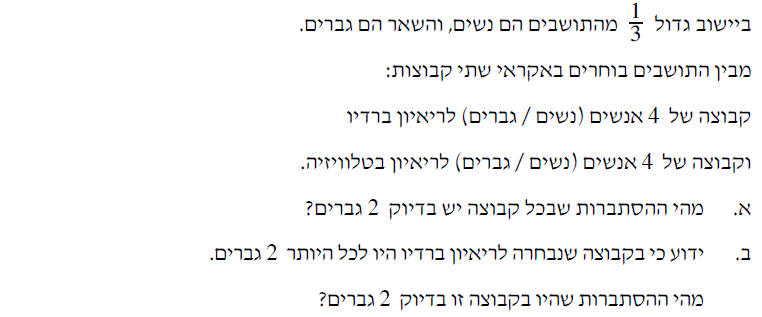
\includegraphics[width=.85\textwidth]{winter-2015-3}
\end{center}

המשמעות של "יישוב גדול" היא (כנראה) שאפשר לבחור את שתי הקבוצות בלי לשנות את ההסתברות של 
$\frac{1}{3}$
במהלך הבחירה, למרות שהבחירה היא ללא החזרה.

\textbf{סעיף א}

נסמן ב-%
$G2$
את המאורע של בחירת שני בגברים בקבוצה אחת ונסמן ב-%
$G22$
את המאורע של בחירת שני גברים בשתי הקבוצות. בחירת גבר נקראת הצלחה ולכן נשתמש בנוסחת ברנולי כדי לקבל את ההסתברות
\textbf{לבדיוק}
שתי הצלחות בקבוצה אחת:
\[
P(G2)={4 \choose 2}\left(\frac{2}{3}\right)^2\left(1-\frac{2}{3}\right)^2=\frac{8}{27}\,.
\]
לפי ההנחה שאין שינוי בהסתברות של הבחירה בין שתי הקבוצות, נקבל:
\[
P(G22)=P(G2)\cdot P(G2)=\frac{64}{729}\,.
\]

\textbf{סעיף ב}

נסמן את המאורע "לכל היותר שני גברים" ב-%
$G012$.
הניסוח
"\textbf{ידוע כי}"
מכוון להסתברות מותנית:
\begin{eqn}
P(G2/G012)&=&\frac{P(G2 \:\cap\: G012)}{P(G012)}\\
\end{eqn}
$G2\subseteq G012$
ולכן המנה היא
$G2=\frac{8}{27}$.
"לכל היותר שני גברים" הוא הסכום של שלוש נוסחאות ברנולי:
\[
\left(\frac{2}{3}\right)^0\left(\frac{1}{3}\right)^4 + {4\choose 1}\left(\frac{2}{3}\right)^1\left(\frac{1}{3}\right)^3 + {4\choose 2}\left(\frac{2}{3}\right)^2\left(\frac{1}{3}\right)^2=\frac{11}{27}\,
\]
והתשובה לשאלה היא:
\[
P(G2/G012)=\frac{\frac{8}{27}}{\frac{11}{27}}=\frac{8}{11}\,.
\]


% !TeX root = probability.tex

%%%%%%%%%%%%%%%%%%%%%%%%%%%%%%%%%%%%%%%%%%%%%%%%%%%%%%%%%%%%%

\section{קיץ תשע"ד מועד ב}

\begin{center}
\selectlanguage{english}
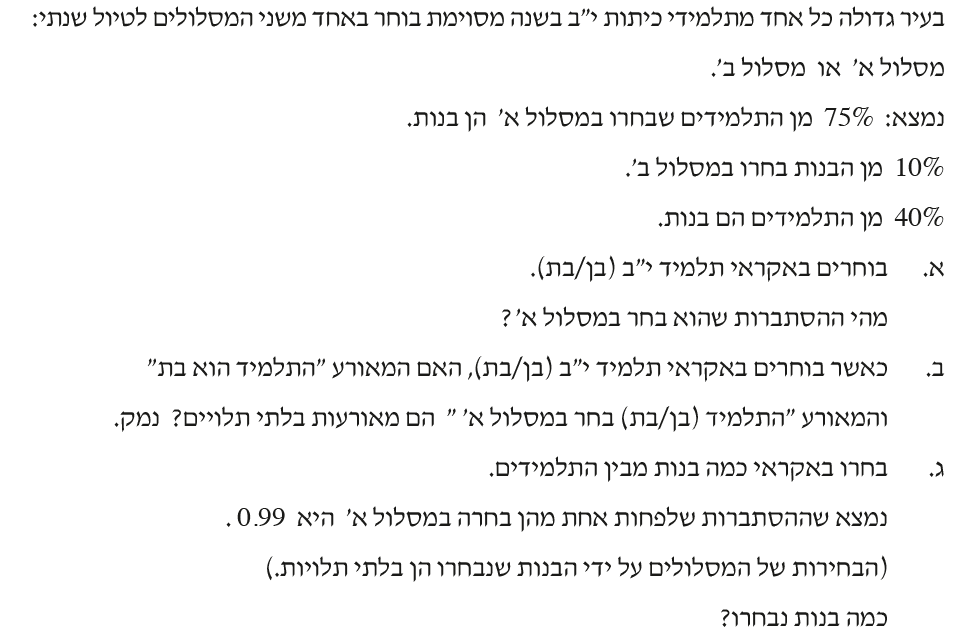
\includegraphics[width=.95\textwidth]{summer-2014b-3}
\end{center}

נמסן את הקבוצות בשאלה:
$G$ \L{(girl)}, $B$ \L{(boy)},
$MA$ \L{(maslul aleph)}, $MB$ \L{(maslul bet)}.
בגלל שיש שני זוגות של קבוצות נציג את ההסתברויות בטבלה. את הטבלה נמלא בשתי דרכים שונות, תחילה ישירות מהנתונים ואחר כך תוך שימוש בהסתברות מותנית.
\begin{center}
\selectlanguage{english}
\begin{tikzpicture}[scale=1.4]
\draw (0,0) grid (3,3);
\node at (2.5,3.3) {$G$};
\node at (1.5,3.3) {$B$};
\node at (3.6,2.5) {$MA$};
\node at (3.6,1.5) {$MB$};
%\node at (2.5,2.7) {$.4-.04=$};
\node at (2.5,2.5) {$.36$};
%\node at (0.5,2.7) {$.36/.75=$};
\node at (0.5,2.5) {$.48$};
%\node at (1.5,2.7) {$.48-.36=$};
\node at (1.5,2.5) {$.12$};
%\node at (0.5,1.7) {$1-.48=$};
\node at (0.5,1.5) {$.52$};
\node at (0.5,0.5) {$1$};
%\node at (1.5,0.7) {$1-.4=$};
\node at (1.5,0.5) {$.60$};
%\node at (2.5,0.7) {\bfseries \R{נתון}};
\node at (2.5,0.5) {$0.40$};
%\node at (1.5,1.7) {$.52-.04=$};
\node at (1.5,1.5) {$.48$};
%\node at (2.5,1.7) {$.1\times .4=$};
\node at (2.5,1.5) {$.04$};
\end{tikzpicture}
\end{center}

\textbf{דרך א'}

נתון ש-% 
$P(G)=0.40$
ונתון ש-%
$10\%$
מהם בחרו במסלול ב', ולכן 
$P(G\cap MB)= .04$,
ומהסתברות משלימה
$P(G\cap MA)= .36$.
הנתון האחרון הוא ש-%
$0.75 P(MA) = 0.36$
ולכן 
$P(MA)=0.36/0.75=0.48$.
את שאר התאים ניתן למלא מהסתברויות משלימות.

\textbf{דרך ב'}

שוב נמלא את התא הימני למטה ב-%
$P(G)=0.40$.
נמשיך:
\begin{eqnarray*}
P(MB/G) &=& \frac{P(MB \:\cap\: G)}{P(G)}=0.10\\
P(MB \:\cap\: G) &=& P(G)P(MB/G) = 0.40\cdot 0.10 = 0.04\,.
\end{eqnarray*}
עוד הסתברות מותנית:
\begin{eqnarray*}
P(G/MA) &=& \frac{P(G \:\cap\: MA)}{P(MA)}=0.75\\
P(MA) &=& \frac{P(G \:\cap\: MA)}{P(G/MA)}=\frac{0.36}{0.75}=0.48\,,
\end{eqnarray*}
ונמלא את שאר התאים באמצעות הסתברויות משלימות.

\textbf{סעיף א}

$P(MA)=0.48$.

\textbf{סעיף ב}
\begin{eqnarray*}
P(G\cap MA) &=&0.36\\
P(G)P(MA)&=&0.40\cdot 0.48=0.19\,.
\end{eqnarray*}
$0.36\neq 0.19$
ולכן המאורעות אינם בלתי תלויים.

\textbf{סעיף ג}

ניתן לחשב "לפחות אחת" על ידי חישוב הסתברות של "אף אחת". ההסתברות שבת לא תבחר מסלול א' היא ההסתברות שהיא תבחר מסלול ב':
\begin{eqnarray*}
P(MB/G) &=& \frac{P(MB \:\cap\: G}{P(G)}= \frac{0.04}{0.40}=0.10\\
(0.10)^n&=&1-0.99=0.01\\
n&=&2\,.
\end{eqnarray*}

%%%%%%%%%%%%%%%%%%%%%%%%%%%%%%%%%%%%%%%%%%%%%%%%%%%%%%%%%%%%%%%%%%%

\section{קיץ תשע"ד מועד א}

\begin{center}
\selectlanguage{english}
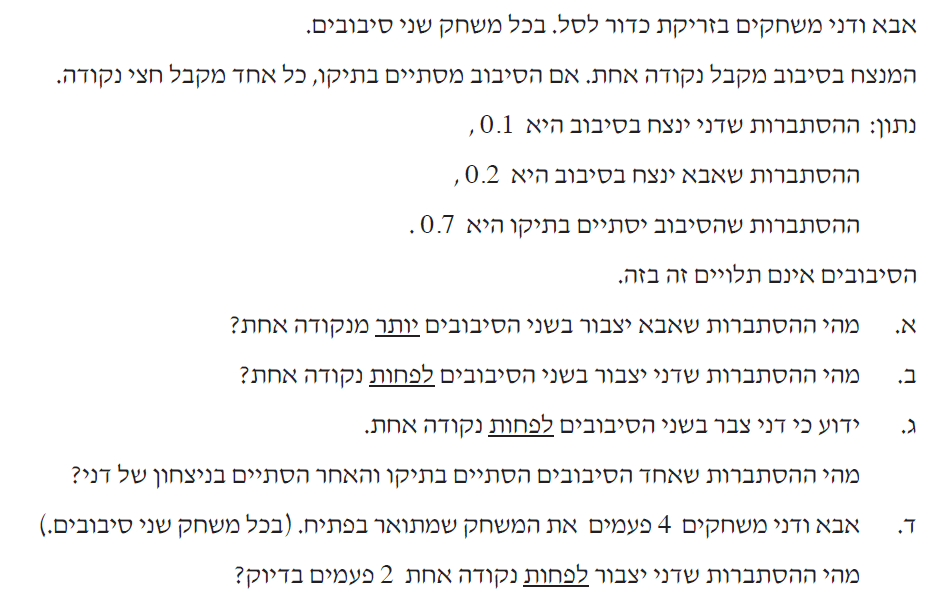
\includegraphics[width=.9\textwidth]{summer-2014a-3}
\end{center}

נסמן ב-%
$D1, D2$ \L{(dani)}
את המאורע שדני מנצח בסיבוב אחד או שניים, נסמן ב-%
$A1, A2$ \L{(abba)}
את המאורע שאבא מנצח בסיבוב אחד או שניים, ונסמן ב-%
$T1, T2$ \L{(teku)}
את המאורע שיהיה תיקו בסיבוב אחד או שניים. השאלה שואלת על סדרה של שני סבבים וזה מכוון לעץ הסתברויות (בעמוד הבא). בסוף כל מסלול רשום מספר הנקודות שאבא צבר ומספר הנקודות שדני צבר.

\begin{figure}
\begin{center}
\selectlanguage{english}
\begin{tikzpicture}
[align=left,grow=right,
level 1/.append style={level distance=3cm,sibling distance=9em},
level 2/.append style={level distance=4cm,
                       sibling distance=3.5em}]
\node[left] {$0$} % root
child {
  node[right] {$\frac{1}{2}$}
    child {
      node[below right,xshift=10pt,yshift=4pt] {$(i) A2=1,D2=1$}
      edge from parent node[below,yshift=-1mm] {$0.7$}
    }
    child {
      node[right,xshift=10pt] 
        {$(h) A2=\frac{1}{2},D2=\frac{1}{2}$}
      edge from parent node[below,xshift=4mm] {$0.1$}
    }
    child {
      node[right,xshift=10pt] 
        {$(g) A2=1\frac{1}{2},D2=\frac{1}{2}$}
      edge from parent node[above,yshift=1mm] {$0.2$}
    }
    edge from parent 
      node[below,xshift=-4mm,yshift=-3mm] {\R{תיקו} $0.7$}
}
child {
  node[right] {$0$}
    child {
      node[right,xshift=10pt] 
        {$(f) A2=\frac{1}{2},D2=1\frac{1}{2}$}
      edge from parent node[below,yshift=-1mm] {$0.7$}
    }
    child {
      node[right,xshift=10pt] {$(e) A2=0,D2=2$}
      edge from parent node[below,xshift=4mm] {$0.1$}
    }
    child {
      node[right,xshift=10pt] {$(d) A2=1,D2=1$}
      edge from parent node[above,yshift=1mm] {$0.2$}
    }
    edge from parent 
      node[below] {\R{דני} $0.1$}
}
child {
  node[right] {$1$}
    child {
      node[right,xshift=10pt] {$(c) A2=1\frac{1}{2},D2=\frac{1}{2}$}
      edge from parent node[below,yshift=-1mm] {$0.7$}
    }
    child {
      node[right,xshift=10pt] {$(b) A2=1,D2=1$}
      edge from parent node[below,xshift=4mm] {$0.1$}
    }
    child {
      node[above right,xshift=10pt] {$(a) A2=2, D2=0$}
      edge from parent node[above,yshift=1mm] {$0.2$}
    }
    edge from parent
       node[above,xshift=-4mm,yshift=3mm] {\R{אבא} $0.2$}
};
\end{tikzpicture}
\end{center}
\end{figure}

\textbf{סעיף א}

במסלול בהם אבא צובר יותר מנקודה אחת הם
\L{(a), (c), (g)},
וההסתברות היא:
\[
P(A2>1)=0.2\cdot 0.2 \,+\, 0.2\cdot 0.7 \,+\, 0.7\cdot 0.2 \,=\,0.32\,.
\]


\textbf{סעיף ב}

המסלולים בהם דני צבר לפחות נקודה אחת הם
\L{(b), (d), (e), (f), (h), (i)}
וההסתברות היא:
\[
P(D2\geq 1)=0.2\cdot 0.1 \,+\,0.1\cdot 0.2 \,+\, 0.1\cdot 0.1 \,+\,0.1\cdot 0.7 \,+\, 0.7\cdot 0.1\,+\,0.7\cdot 0.7\,=\,0.68\,.
\]


\textbf{סעיף ג}

הניסוח "ידוע" מכוון להסתברות מותנית, אבל
$D1\cup T1\subseteq D2\geq 1$
ולכן:
\begin{eqnarray*}
P((D1\cup T1)/D2\geq 1)&=&\frac{P((D1\cup T1) \:\cap\: D2\geq 1)}
  {D2\geq 1}\\
  &=&\frac{P(D1\cup T1)}{D2\geq 1}\\
\frac{0.1\cdot 0.7 \,+\, 0.7\cdot 0.1}{0.68} &=& \frac{7}{34}= 0.2059\,,  
\end{eqnarray*}
כי המסלולים המתאימים הם 
\L{(f), (h)}.

\textbf{סעיף ד}

נשמתמש בנוסחת ברנולי כי למצוא את ההסתברות לבדיוק פעמיים:
\[
{4\choose 2}P(D2)^2\: (1-P(D2)^2 =
{4\choose 2} (0.32)^2 (0.68)^2= 0.2841\,.
\]

%%%%%%%%%%%%%%%%%%%%%%%%%%%%%%%%%%%%%%%%%%%%%%%%%%%%%%%%

\section{חורף תשע"ד}

\begin{center}
\selectlanguage{english}
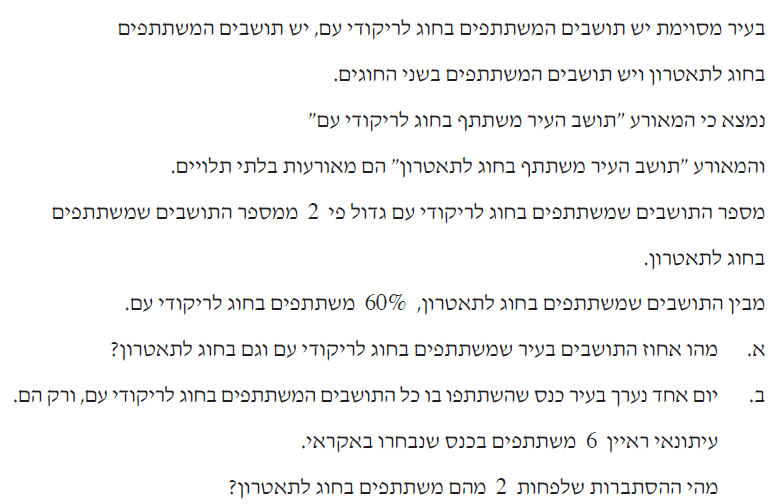
\includegraphics[width=.9\textwidth]{winter-2014-3}
\end{center}

נסמן ב-%
$T$ \L{(theatron)}
את המשתתפים בתאטרון ונסמן ב-%
$R$ \L{(rikudei)}
את המשתתפים בריקודי עם. המילה "מבין" מכוונת להתסברות מותנית. ההסתברויות הן של זוגות של מאורעות ולכן נשתמש בטבלה.


נתון
$P(R/T)=0.6$
ושהאירועים בלתי תלויים. נחשב:
\[
P(R/T)=\frac{P(R\cap T)}{P(T)}=\frac{P(R)\cdot P(T)}{P(T)}=P(R)=0.06\,.
\]
ביחד עם הנתון
$P(R)=2P(T)$
נתחיל למלא את הטבלה:
\begin{center}
\selectlanguage{english}
\begin{tikzpicture}[scale=1.4]
\draw (0,0) grid (3,3);
\node at (2.5,3.3) {$T$};
\node at (1.5,3.3) {$\overline{T}$};
\node at (3.3,2.5) {$R$};
\node at (3.3,1.5) {$\overline{R}$};
\node at (0.5,2.5) {$0.60$};
\node at (2.5,0.5) {$0.30$};
\node at (.5,.5) {$1.0$};
\node at (1.5,.5) {$0.70$};
\node at (.5,1.5) {$0.40$};
\end{tikzpicture}
\end{center}
שוב נסתמך על העובדה שהאירועים בלתי תלויים ונקבל:
\[
P(R\cap T)=P(R)\cdot P(T)=0.60\cdot 0.30=0.18\,,
\]
וניתן למלא את הטבלה לפי הסתברויות משלימות:
\begin{center}
\selectlanguage{english}
\begin{tikzpicture}[scale=1.4]
\draw (0,0) grid (3,3);
\node at (2.5,3.3) {$T$};
\node at (1.5,3.3) {$\overline{T}$};
\node at (3.3,2.5) {$R$};
\node at (3.3,1.5) {$\overline{R}$};
\node at (2.5,2.5) {$0.18$};
\node at (0.5,2.5) {$0.60$};
\node at (1.5,2.5) {$0.42$};
\node at (0.5,1.5) {$0.40$};
\node at (0.5,0.5) {$1.0$};
\node at (1.5,0.5) {$0.70$};
\node at (2.5,0.5) {$0.30$};
\node at (1.5,1.5) {$0.28$};
\node at (2.5,1.5) {$0.12$};
\end{tikzpicture}
\end{center}

\textbf{סעיף א}

$P(R\cap T)=0.18$.

\textbf{סעיף ב}

הניסוח "כל התושבים המשתתפים בחוג לריקודי עם, ורק הם" מכוונות להסתברות מותנית:
\[
P(T/R) = \frac{P(T\cap R)}{P(R)} = \frac{P(T)P(R)}{P(R)}= P(T)=0.30\,.
\]
כדי לחשב "לפחות שניים" נשתמש בנוסחת ברנולי ונחשב את המשלים ל-"אפס או אחד":
\[
P(T\geq 2/R)=1-{6\choose 0}(0.3)^0(0.7)^6 -{6\choose 1}(0.3)^1(0.7)^5=0.5798\,.
\]

% !TeX root = probability.tex

%%%%%%%%%%%%%%%%%%%%%%%%%%%%%%%%%%%%%%%%%%%%%%%%%%%%%%%%

\section*{המלצות}

\addcontentsline{toc}{section}{\large המלצות}

\begin{itemize}
\item
קרא בזהירות את השאלות. לעתים הן ארוכות וחשוב להבין את המשמעות של כל פסקה.

\item
כמעט כל הבחינות מכילות שאלות על הסתברות מותנית. ניסוחים רבים מכוונים להסתברות מותנית וחשוב להכיר אותם!

\begin{itemize}
\item
הניסוח השכיח ביותר משתמש במילים
"\textbf{אם ידוע ש-}"
או
"\textbf{ידוע כי}".

\item
בבחינה של חורף תשע"ז כתוב "%
\textbf{אם} $\ldots$ ,
\textbf{מהי ההסתברות} $\ldots$".
לא לגמרי ברור שלמילה "אם" יש משמעות של "אם ידוע", אבל זאת הכוונה.

\item
לעתים קרובות )בחינה של קיץ תשע"ה ב'( כתוב "%
\textbf{מה ההסתברות לבחור} $\ldots$
\textbf{מבין} $\ldots$".

\item
יוצא מן הכלל: בבחינה של קיץ תשע"ו א' כתוב
"\textbf{מבין}
כל הנבחנים". המילה "מבין" בדרך כלל מכוונת להסתברות מותנית, אבל כאשר "מבין" מתייחס ל-%
"\textbf{כל}
הנבחנים", אין הסתברות מותנית. לחילופין אפשר לחשב הסתברות מותנית כאשר החיתוך מצטמצם:
\[
P(X/\textrm{\R{כל הנבחנים}})=
\frac{P(X\cap \textrm{\R{כל הנבחנים}})}
{P(\textrm{\R{כל הנבחנים}})} = 
\frac{P(X)}{1}=P(X)\,.
\]

\item
בבחינה של קיץ תשע"ח א' הניסוח הוא: "%
$n\%$
נעזרו בחבריהם 
$N$
ו-%
$\displaystyle\frac{k}{n}$
\textbf{מהם}
עברו את הבחינה
$A$".
ברור ש-%
$P(A\cap N) = k$,
אבל נבדוק לפי הנוסחה להסתברות מונתית:
\begin{eqnarray*}
P(A/N) &=& \frac{P(A\cap N)}{P(N)} = \frac{k}{n}\\
P(A\cap N)&=&k\,.
\end{eqnarray*}

\item
בבחינה של חורף תשע"ד יש ניסוח אחר: "כל התושבים המשתתפים ב-
$\ldots$,
\textbf{ורק הם}".
\end{itemize}

%%%%%%%%%%%%%%%%%%%%%%%%%%%%%%%%%%%%

\item
כאשר יש חיתוך בחישוב של הסתברות מותנית, לעתים קרובות ניתן לפשט את החישוב. בבחינה של קיץ תשע"ז א' יש לחשב
$P(D=4\cap D\ge 3)$,
אבל אם ערך גדול או שווה
$3$
\textbf{וגם}
שווה ל-%
$4$,
אז הוא שווה ל-%
$4$, 
ולכן מספיק לחשב
$P(D=4)$.

%%%%%%%%%%%%%%%%%%%%%%%%%%%%%%%%%%%%

\item
אם שני אירועים בלתי תלויים, חישוב ההסתברות המותנית מצטמצם:
\[
P(A/B) = \frac{P(A\cap B)}{P(B)} = \frac{P(B)\cdot P(A)}{P(A)}= P(B)\,.
\]
מצב זמ מופיע בבחינות של חורף תשע"ז, חורף משע"ח, קיץ תשע"ה א', חורף תשע"ד.
%%%%%%%%%%%%%%%%%%%%%%%%%%%%%%%%%%%%



\item
המילה 
\textbf{בדיוק}
מכוונת לחישוב אחד של נוסחת ברנולי, כי נתון כמה "הצלחות" צריכות להיות וגם כמה "כשלונות".

%%%%%%%%%%%%%%%%%%%%%%%%%%%%%%%%%%%%

\item
בבחינה של קיץ תשע"ז א' כתוב "%
\textbf{בוחרים באקראי}
$\ldots$,
\textbf{עד של-}
$3$
מהם
\textbf{בדיוק}
יש קלנועית". המשמעות של "עד ש-" היא שמפסיקים את הבחירה האקראית כאשר הבחירה 
\textbf{האחרונה} 
היא "הצלחה". במקרה זה נשארו שתי "הצלחות" שיש לחשב את ההסתברות שלהן לפי נוסחת ברנולי, ואז להכפיל בהסתברות של "הצלחה" בבחירה האחרונה:
\[
\overbrace{\pm\;\pm\;\pm\;\pm\;\pm}^{2/5}\quad\quad \overbrace{+}^{1/1}\,.
\]

%%%%%%%%%%%%%%%%%%%%%%%%%%%%%%%%%%%%

\item
בבחינה של קיץ תשע"ז ב' הביטוי "מוציאים באקראי
$\ldots$",
ובהמשך הביטוי "מוציאים באקראי
\textbf{שוב}
$\ldots$"
מכוון לשימוש בעץ כדי לתאר את הבחירה הסדרתית.

%%%%%%%%%%%%%%%%%%%%%%%%%%%%%%%%%%%%

\item
בבחינה של קיץ תשע"ח א' המשמעות של הניסוח "%
\textbf{לפחות אחת}
משתי הטענות I, II היא שהאירוע קורה אם קורה אחד מהאירועים I, II,
\textbf{או שניהם},
המסומן I
$\cup$
II".
יש שתי דרכים לחשב את ההסתברות:
\begin{eqnarray*}
P(\textrm{I} \cup \textrm{II}) &=& P(\textrm{I}) + P(\textrm{II}) - P(\textrm{I} \cap \textrm{II})\\
P(\textrm{I} \cup \textrm{II}) &=& P(\textrm{I}-\textrm{II}) + P(\textrm{II}-\textrm{I}) + P(\textrm{I} \cap \textrm{II})\,.
\end{eqnarray*}

%%%%%%%%%%%%%%%%%%%%%%%%%%%%%%%%%%%%

\item
בבחינה של  קיץ תשע"ח ב' יש לחשב את ההסבתרות לפי נוסחת ברנולי
${n \choose k}p^k(1-p)^{n-k}$.
\begin{itemize}
\item
אם
$k=0$
אזי
${n\choose 0}=1$
והנוסחה מצטמצמת ל-%
$p^0(1-p)^{n-0}=(1-p)^n$.
\item 
אם
$k=n$
אזי
${n\choose n}=1$
והנוסחה מצטמצמת ל-%
$p^n(1-p)^{n-n}=p^n$.
\end{itemize}


%%%%%%%%%%%%%%%%%%%%%%%%%%%%%%%%%%%%

\item
בבחינות של קיץ תשע"ו א' ו-ב' יש שלוש תוצאות לפעולה במקום שתיים. סכום ההסתברויות חייב להיות אחד, ולכן כאשר מחשבים משלים להסתברות אחת, יש להחסיר את שתי ההסתברויות האחרות. בבחינה של מועד ב' ההסתברות לתיקו היא אחד פחות ההסתברות שיעל תנצח פחות ההסתברות אנה תנצח:
\[
P(\textrm{\R{תיקו}}) =
1 - (P(\textrm{\R{יעל}})+
P(\textrm{\R{אנה}})) = 
1 - P(\textrm{\R{יעל}})-
P(\textrm{\R{אנה}}) \,.
\]

\item 
במספר בחינות (חורף תשע"ה, קיץ תשע"ד ב', קיץ תשע"ה ב') מתואר מצב הנקרא "שליפה ללא החזרה". אם יש מספר נמוך של תושבים, השליפות לא בלתי-תלויות. כאשר כתוב "ישוב גדול", "עיר גדולה", "אוניברסיטה גדולה", אני מניח שכוונה שיש מספר כל כך גדול של תושבים שאין שינוי משמעותי בהסתברות משליפה אחת לבאה אחריה.
\end{itemize}


\end{document}
